\documentclass[11pt]{article}
\usepackage{amsmath,textcomp,amssymb,graphicx,enumerate}
\usepackage{tikz}
\usepackage{float}
\usepackage{caption}
\usepackage{epsfig,graphicx}
\usepackage{palatino}
\usepackage{fancybox}
\usepackage{hyperref}
\usepackage{url}
\usepackage{ctex}
\usepackage[procnames]{listings}
\usepackage{multicol}
\usepackage{pdfpages}
\usepackage{calc}
\usepackage[usestackEOL]{stackengine}
\usetikzlibrary{automata,positioning, arrows}
\usetikzlibrary{shapes}
\usetikzlibrary{positioning, quotes}
\newcommand{\chinesedash}{\rule[.7ex]{\widthof{二字}}{0.5pt}}
% "define" Scala
\usepackage[T1]{fontenc}  
\usepackage[scaled=0.82]{beramono}  
\usepackage{microtype} 

\sbox0{\small\ttfamily A}
\edef\mybasewidth{\the\wd0 }

\lstdefinelanguage{scala}{
  morekeywords={abstract,case,catch,class,def,%
    do,else,extends,false,final,finally,%
    for,if,implicit,import,match,mixin,%
    new,null,object,override,package,%
    private,protected,requires,return,sealed,%
    super,this,throw,trait,true,try,%
    type,val,var,while,with,yield},
  sensitive=true,
  morecomment=[l]{//},
  morecomment=[n]{/*}{*/},
  morestring=[b]",
  morestring=[b]',
  morestring=[b]"""
}

\usepackage{color}
\definecolor{dkgreen}{rgb}{0,0.6,0}
\definecolor{gray}{rgb}{0.5,0.5,0.5}
\definecolor{mauve}{rgb}{0.58,0,0.82}

% Default settings for code listings
\lstset{frame=tb,
  language=scala,
  aboveskip=3mm,
  belowskip=3mm,
  showstringspaces=false,
  columns=fixed, % basewidth=\mybasewidth,
  basicstyle={\small\ttfamily},
  numbers=none,
  numberstyle=\footnotesize\color{gray},
  % identifierstyle=\color{red},
  keywordstyle=\color{blue},
  commentstyle=\color{dkgreen},
  stringstyle=\color{mauve},
  frame=single,
  breaklines=true,
  breakatwhitespace=true,
  procnamekeys={def, val, var, class, trait, object, extends},
  procnamestyle=\ttfamily\color{red},
  tabsize=2
}

\lstnewenvironment{scala}[1][]
{\lstset{language=scala,#1}}
{}
\lstnewenvironment{cpp}[1][]
{\lstset{language=C++,#1}}
{}
\lstnewenvironment{bash}[1][]
{\lstset{language=bash,#1}}
{}
\lstnewenvironment{verilog}[1][]
{\lstset{language=verilog,#1}}
{}



\lstset{frame=, basicstyle={\footnotesize\ttfamily}}

\newcommand{\todo}[1]{\emph{TODO: #1}}
\newcommand{\comment}[1]{\emph{Comment: #1}}
\def\Name{ 周盈坤 }  % Your name
\def\SID{2015K8009929023}  % Your student ID number
\def\le{\leqslant}
\def\logN{\log{}n}
\newcommand{\ro}[1]{\romannumeral #1}
\def\Session{Fall 2018}

% uncomment following for final submission
\renewcommand{\todo}[1]{}
\renewcommand{\comment}[1]{}

\newenvironment{qparts}{\begin{enumerate}[{(}a{)}]}{\end{enumerate}}
\def\endproofmark{$\Box$}
\newenvironment{proof}{\par{\bf Proof}:}{\endproofmark\smallskip}

\textheight=9in
\textwidth=6in
\topmargin=-.75in
\oddsidemargin=0.25in
\evensidemargin=0.25in


\begin{document}
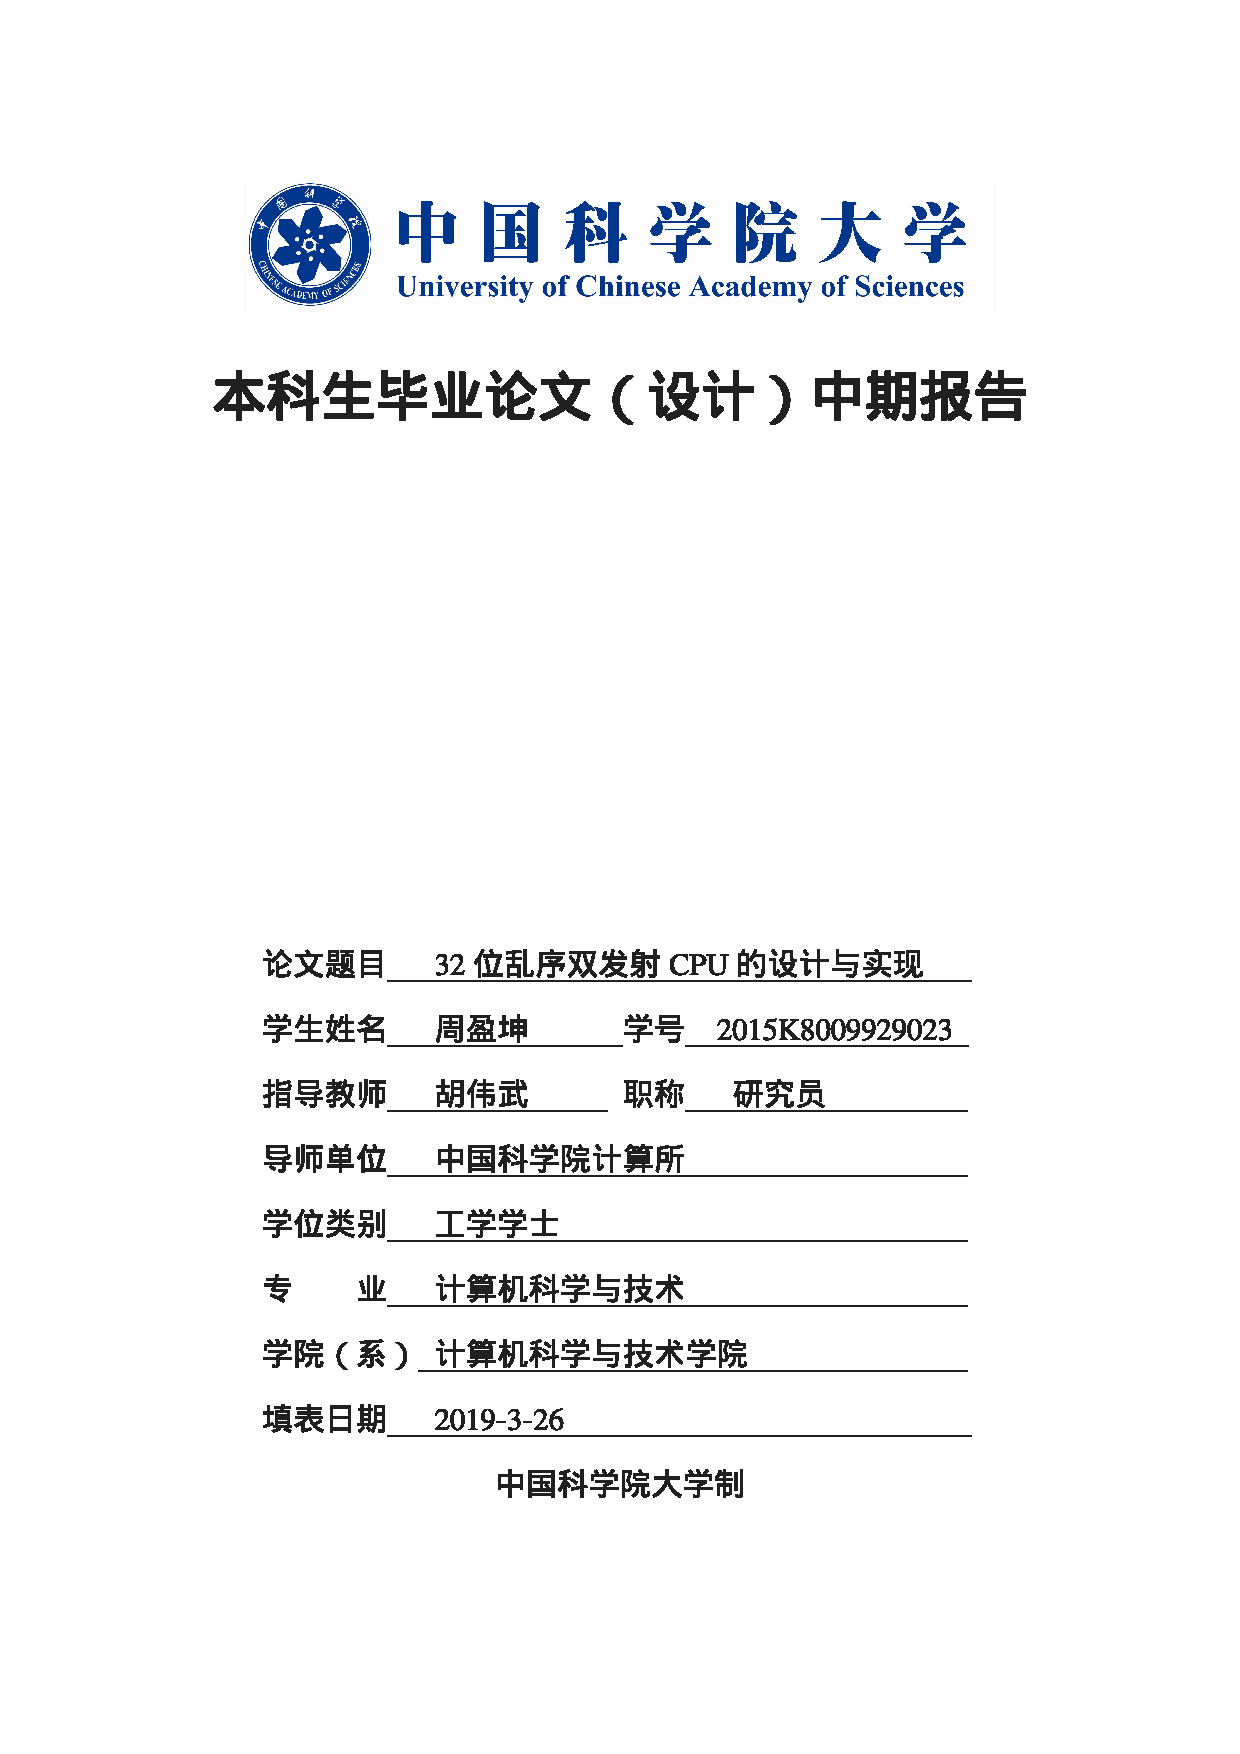
\includepdf[pages={1,2},scale=1.1]{zhongqi.pdf}
\section{摘要}
本论文旨在分析探讨中采用乱序、多发射、超标量技术的高性能通用处理器结构设计,以及对其性能的考量与取舍,并最后自主设计出一款能够运行简单嵌入式程序的高性能乱序双发射处理器。相较于经典的五级流水,乱序多发射以及超标量的引入无疑会大大增加处理器的复杂度,所以如何有效的控制设计的复杂度,在毕业设计这么短的时间内就能够设计出一款能够运行程序的高性能处理器就必须有所简化,以便集中力量进行最为核心的超标量发射以及乱序调度的设计。所以最后简化的内容方法如下:首先ISA指令集采用了目前最为精简的RISC-V中RV32I指令集总共47条指令,包括用户态指令和特权态指令而不是之前比较熟悉的MIPS;其次编写的语言采用由加州大学伯克利分校设计开发的Chisel硬件描述语言来提高设计的效率以及控制设计的复杂度而不是之前较为熟悉的Verilog;最后运行的程序也是相对简单的诸如Dhrystore和Coremark的嵌入式程序,而不是spec2000或者spec2006这样需要运行在操作系统环境下的大型程序。
%TODO成果与结论

%TODO相比于经典的单发射五级流水处理器,为了进一步提高处理器性能而引入的乱序多发射多发射技术使得处理器的设计变得非常复杂。但是无论从哲学或者工程学的角度来看,高效的事物往往又是简洁的。
%TODO:scala, chisel是强类型的, 利用编译
%TODO对性能影响最大的是load+branch组合 对高性能的衡量基本上限定在IPC上

\section{目录}

%%%%%%%正文
\section{绪论}
%选题的背景、意义、目的、研究范围、本论文所要解决的问题等
经典的单发射五级流水处理器在高性能的需求面前早已遇到了瓶颈,同时随着集成电路晶体管数量的不断增加,能够有更多的资源来支持更为复杂的单核处理器的设计实现,其中就包括了乱序调度,超标量发射和指令缓存,将处理器的性能从五级流水的上限中解放出来,在存储墙愈加严重的现状下依然能够得到性能的提升。选题的目的在于通过自主地设计出一款乱序双发射处理器初级模型的过程,积累设计高性能处理器的宝贵经验,体会突破单发射五级流水的性能极限之后再不断的提高处理器执行指令效率的过程是非常有意义的。但是这是一个庞大的工程,个人半年的时间很难做完,对于研究的范围和所要解决的问题就要做出相应的简化。研究的范围大体框架是实现一个乱序调度,超标量宽度为2的处理器设计,但是一些实现的细节可以做出一些不属于核心内容范畴的简化,如由于32位架构比64位架构简单故采用32位的架构;MMU可以暂时不做;特权指令的实现可以相应从简;操作系统的移植也暂时不需要;指令集选用的是最简单的RISC-V RV32I子集;编程语言选用抽象等级更高的Chisel。所以概括起来就是实现一个基于RV32I指令集的32位,不带MMU,
带icache和dcache这两个分离式的一级cache并支持延迟访存AXI总线的运行在Machine Mode下的乱序双发射处理器。像乱序双发射,L1cache和延迟访存总线这些最为核心的要素全部都保留住。索要解决的问题也就集中在如何在提高取指带宽的同时更好的调度指令的执行已达到接近于理论上最优的性能峰值。
\section{研究背景}
近年来,RISC-V开源体系结构的兴起,使得很多软硬件实力相对于大公司薄弱很多的研究个体受益良多。RISC-V开源的项目越来越多,有微处理器设计的如Rocket和BOOM;有更抽象的电路描述语言的如Chisel;也有针对 RISC-V的模拟器如Spike可以在上面调试软件,或者得到程序的执行写回信息从而用来调试处理器;还有已经移植成功的上层软件栈如Linux,GCC和LLVM。这些开源的项目大大降低了研究个体独立设计出一款高性能处理器以及在上面运行软件栈的难度与门槛。对于毕业设计而言,能够在短短3个月的时间内就设计出一款成型的双发射乱序流水线处理器,很大程度上正是归功于RISC-V的开源项目兴起的背景。从指令集ISA,编程语言,开源项目三个角度来看,RISC-V开源体系结构对于毕业设计都有很多的帮助。
\subsection{MIPS和RISC-V}
设计一款具体的CPU要对应于具体的ISA,有两个较为简单的指令集可供选择:一个是MIPS的MIPS32子集,一个是RISC-V的RV32I子集,两者都是RISC的典型ISA。MIPS体系结构从最开始1985年推出的第一代指令集MIPS I以及其R2000处理器,已经有三十多年的历史;而RISC-V作为加州大学伯克利分校的RISC系列的第五代指令集,在伯克利分校大力推广下成为了近年来热度最高的开源指令集。设计中最后选择RV32I而不是MIPS32有多方面的考虑。首先是处于对于新事物的好奇和新鲜感,其次由于本科的教学的参考ISA就是MIPS,通过本科的学习和工程实践对于MIPS的有了初步的认识,也能够体察到MIPS在ISA设计中的一些缺陷。比如延迟槽的引入,这个当初对单发射五级流水从体系结构上做出的优化被日后的工程实践证明是一个历史的包袱。因为分支指令后面紧跟一条延迟槽的设计仅仅适用于像单发射五级静态流水这样的简单的设计中,超标量的高性能处理器取指仍然需要做转移猜测,所以延迟槽的引入反而增加了高性能处理器取指和中断例外设计的复杂度。另外,为了存储定点乘除法结果而单独加入的HILO寄存器,再通过MFHI,HFLO,MTHI,MTLO这四条指令与通用寄存器对进行交互也会增加处理器设计的复杂度。如果继续深入分析,MIPS的特权态的设计会显得很凌乱,对于特权模式的处理机制有是逐渐增量加入的方式,并不是一开始就规划地非常清楚,欠缺章法体系;同时在80年代MIPS诞生之初也没有考虑到64为虚拟地址空间的需求和嵌入式领域的指令压缩的需求,但是指令空间设计考虑不周,64位尚能够与32位兼容,但是为了嵌入式压缩指令而引入的microMIPS就是重新设计的与原有的MIPS 32/64并不兼容。所以比MIPS晚诞生20多年的RISC-V能够站在后来者的角度审视借鉴之前诞生的众多指令集的优缺点,毕竟ISA体系结构的演进发展已经有40多年的历史了,一些基础的设计都趋向于收敛,所以RISC-V能够从一开始就有一套清晰的设计规划,摒弃了很多包括之前提及的MIPS设计中的缺陷,做到32位,64位,压缩变长指令集很好的统一,以简洁优美的形式呈现,最大化的简化了硬件指令译码器的逻辑。同时因为有了系统的规划,虽然目前特权态的有些规定还不是那么明确,高性能的SIMD指令亦或是向量指令也不完善,但是对于处理器运行的模式确实非常明确有章法,指令编码空间设计合理使得指令的可拓展性极强以便日后之需。下面通过对比MIPS来具体分析RISC-V的特点以及简洁优美的设计考量。
\subsection{Verilog和Chisel}
设计的实现是将逻辑层面抽象的想法概念用具体的语言严谨地描述出来,所以设计处理器这样的硬件就需要硬件的描述语言。当今主流的描述语言仍是90年代开发的Verilog。该语言设计参考的是C语言,最开始设计出来用作电路功能的仿真,因而有很多语法只适用于软件的仿真,不能作为物理电路的综合布局布线。可被综合的最常用的语句是组合逻辑的assign语句块和时序逻辑的同步always语句块。事实上这两种语句组合就能够满足绝大多数的电路设计的需求,其中就包括双发射乱序处理器。但是就像能够描述所有软件程序的汇编语言一样,Verilog的抽象等级太低,细节太多,描述电路的能力先天不足,主要体现在语句的逻辑集成度不高,时常一个简单的逻辑代码量却不少;变量名、函数名的管理机制非常原始,甚至都没有像C语言的struct结构体这种集成化的设计,管理起来相当麻烦;常用的简单逻辑代码复用度不高,代码复用基本上只能用Module这样一种单一的写法;对多维的向量数组描述支持不足;参数的管理同样繁琐落后。所以原本逻辑已经非常复杂的双发射乱序处理器采用Verilog来描述,又会因为语言层面的弱势,使得实现起来会异常的繁琐,复杂度得不到控制。对像乱序多发射处理器这样的大工程的搭建、调试以及持续的优化、增量式演进都带来不小的挑战。

Chisel没有那么神秘,并不是变革性的另一套硬件描述,而是包装在verilog之上具有面向对象和函数化编程的脚本语言,是一种以verilog中上述两种语句为基本块的更上一层的抽象。多一层的抽象就是为了解决Verilog表示能力不足的缺陷,比如面向对象里的类和对象、接口以及多态与继承的特性,可以很好的复用代码,对变量名和方法名以及参数名的管理更加有条理;另外函数式的编程如lambda函数可以用来很便捷的描述简单的电路逻辑。

Chisel之于Verilog就像JAVA之于汇编。Chisel和JAVA都是强类型的语言,在编译的时候会做类型检查,从而避免很多因为类型不当导致的逻辑错误;而Verilog和汇编都是没有类型的概念的,一个32位的逻辑寄存器,汇编可以任意的操作而不用在乎这个寄存器代表的是不是整形或者字符型,同样Verilog对一个32bit的Wire和Reg向量也可以任意操作。正是因为这种毫无约束的操作,使得用汇编或者verilog编程都会比Chisel或者JAVA来得繁琐而易出错。但是略显不同的是,一个初学者可以在不知道汇编语言的情况下就能够掌握JAVA语言这样的抽象等级高的语言,但是却不能在没有熟练运用Verilog中的两个基本语句的前提下掌握Chisel。换言之就是C语言对于汇编的抽象是彻底的,但是Chisel对于Verilog的抽象是不彻底的,所以Chisel适用于有一定硬件设计工程经验的人,而不适用于初次上手设计电路的初学者。
%TODO大部分的bug来自于分支预测错误带来的取消,因为是多线程的程序,所以容易出现没有来得及取消的情况,这一点上要能够举一反三的调bug
\subsection{RISC-V开源项目}
\section{材料与方法}
\section{结果}
\section{讨论}
\section{结论与展望}
%%%%%%%reference
\section*{\huge{一、学位论文进展情况}}
学位论文的工作方面,目前完成了对chisel的熟悉,并用伯克利一个简单开源的处理器设计测试平台完成了基于risc-v32i的单发射五级静态流水和双发射五级静态流水的编写和软件模拟的调试。同时完成了双发射乱序所有代码逻辑的编写以及前端的逻辑验证,正在进行对中间层和后端各个队列的模块级测试与验证。

学位论文的撰写方面,开题报告可以作为学位论文第一二章背景意义论述的参考,而在中期报告中介绍已取得阶段性成果的部分(见下文)可以作为学位论文第三章主体设计论述的参考。接下来第四章可以是处理器功能正确性验证的阐述;第五章写处理器性能评测与分析;最后一章第六章可以是针对第五章性能分析而提出的结构优化。
\section*{\LARGE{存在的问题}}
从中期以后的工作量估计仍然很大,不光要尽快的完成验证,同时还要针对benchmark进行细致的分析、优化。
\section*{\LARGE{已取得的阶段性成果}}
\section{CPU框架\chinesedash 解耦合模型}
这里的框架指的不是单发射顺序五级流水线,不是双发射顺序七级流水线,不是双发射乱序八级流水,而是一种更加通用的解耦合模型--前端(front end), 后端(back end)。
\begin{enumerate}
	\item 前端: 提供稳定的指令流,具体来说就是从初始地址开始源源不断地取回指令提供给后端处理
	\item 后端: 接受来自前端的指令,进行运算,最后写回寄存器堆或者写回memory(寄存器堆可以认为是一个缓存memory数据的很小的cache,但是和一般意义的cache不同的是,查找寄存器堆不需要进行容量差而导致的tag位的比较,而是由指令中相关域指定的全索引)。
\end{enumerate}
这个模型的优势在于:
\begin{enumerate}
	\item 前端不需要关心后端指令执行的机制;后端也不需要在乎前端取指状态机的运转流程以及所采用的缓存策略。例如对于cacheable的区域的取指,可以利用cache提高取指效率也可以不用。
	\item 连接两端之间接口的信号是非常少而且清晰的。屈指可数$\chinesedash$前端到后端方向有指令以及指令是否有效,指令的pc,以及下一条pc的转移猜测;后端向前端有对于指令流的反馈如取回的指令是不是由于流水线的繁忙而需要阻塞,branch/jump类指令和例外中断对于指令流的重定向,以及对于转移预测器的数据结构的更新。
	\item 前后端的解耦合模型,清晰的接口对于功能的调试、性能的调优也大有帮助。
\end{enumerate}

\section{CPU高性能因素考量\chinesedash 通向双发射乱序设计}
衡量高性能的通用处理器有两个维度:频率(电路一周期所需的时间)和IPC(单位周期可以提交的指令数)。不同于IPC维度是硬指标,频率这个维度,不同的硬件实现(FPGA/ASIC),甚至不同的综合工具都会对其有较大的影响,所以一个比较客观的分析是从一个触发器的Q端到下一个触发器的D端最多的门级数(在设计的时候靠着经验进行大致的估算和衡量,但是由于扇入扇出的影响,存在误差),所以现阶段对于高性能的评价更多依据的是IPC的高低。

要做高性能,基于前后端模型可以非常清晰的解耦合为做到高性能的前端、做到高性能的后端。
\begin{enumerate}
	\item 高性能的前端
	
	供应指令要快。这个快又可以继续细分用三个维度来衡量:
	\begin{enumerate}
		\item 能够取回来有效指令的周期占总周期的比重$ \chinesedash $由于现代的处理器运算单元频率越来越快,存储器的频率就相对变慢。直接访问存储器要数十上百周期。优化的方法是引入cache,面积小频率快。
		\item 指令宽度$ \chinesedash $每周期的指令条数,直观上来看,指令宽度越大,指令供应的越快。
		\item 指令的正确率$ \chinesedash $例如在没有延迟槽设计的isa下的较为简单的指令宽度为1的单发射五级静态流水线结构中,当跳转指令还没有运算出来跳转的方向和地址时,若阻塞前端会白白浪费周期数。所以一般会采用各种预测投机策略来续上指令流。对于结构越来越复杂,缓存指令数越来越多的后端,对指令正确率的要求也就越来越高。
	\end{enumerate}
	对照这三个维度,同时还有考虑频率时序的优劣,就有很多权衡考虑$ \chinesedash $cache做多少大,多少路,要有多少个cache行,每个cache行要长度多少。cache的大小首要考虑的是ISA和操作系统对于分页大小的规定,对于RISC-V来说是固定4KB,所以如果cache每路的容量大于4KB,不是实地址低位索引就会有顶着色的问题。但是若采用实地址索引,对于tlb的逻辑将是一个极大的挑战。虚地址要先经过tlb转化为实地址再去索引cache,若做成一个周期时序会紧张,若做成两级流水,由于跳转指令的存在,猜错的时候就会多浪费一个周期,效率反而会下降。一种比较简单的方案是cache单路的容量做成不超过4KB,这样用来索引cache的index作为虚实地址的低位是一致的,换言之tlb转换和cache访问就可以达到并行,也即通过tlb cam表查找得到实地址的高位锁存一拍再和与此时同步cache里读出的tag域做比较得到是否命中的信号。这样cache命中就只需要一拍了。但是代价是cache的容量比起龙芯杯大赛设计的单路64KB的icache容量就显得太小了。出于增大容量的考虑,在毕业设计的CPU中果断准备采用四路的设计,每一路是4KB大小(这样总共就有16KB的容量),其他配置基本上承袭的是大赛的设计,cache行的的长度为64 Byte,可以存放16条4B的指令。
	
	与cache不同,其他两个维度都与后端有着比较紧密的关联。对于指令宽度,如果前端是2条指令的宽度,后端做单发射流水就不合适,指令供应的过快后端消化不掉就会导致流水线阻塞,所以执行单元相应的至少需要两套。其次指令的宽度也不是越大越好,原因有如下几点:
	\begin{enumerate}
		\item 宽度大,会增大前端的逻辑复杂度,同一周期的各个指令非常容易出现前后数据相关、控制相关的问题。
		\item 面向memory的接口宽度仍为一条指令,所以一旦出现cache miss就会有大量的空泡产生
		\item 对转移猜测器产生了巨大的压力,每一周期对宽度内的每一个pc都要做预测,接着还要根据预测的结果再做相应的前面指令无效掉后面指令的逻辑,整个过程电路的延迟很大。而且不光延迟大,取指的效率也不会呈现出正相关。
	\end{enumerate}
	综上所述,我采取的策略就是定下来前端宽度是两条指令,把宽度是两条指令的取指器效率做到极致。
	
	最后是指令的正确性,这个与后端也有着很大的关联。正如前问提到的,后端的结构越复杂,级数越多,缓存的指令越多,如果还支持乱序,那么对于指令的正确性要求越高。一方面是级数越多,跳转指令从取指到执行的周期越长,如果猜错,损失的周期数就越多。换言之提高转移预测的准确性对乱序的提升会比顺序的显著。另外一方面,对转移猜测而言,结构越复杂的后端意味着前端可以有更多的周期进行分级的预测并矫正上游流水级的预测结果,使之更准确。例如处理器的第三级要做rename以及分配物理寄存器而来不及执行,那么这个时候跳转结果依旧没有得到,还能够继续进行预测矫正。
	\item 高性能的后端
	
	指令执行要快。这个``快''可以理解为尽可能少的阻塞前端指令的传送,也就是说不能因为少数的``刺头''指令拖累了整个CPU的指令通路,这里指的主要是load/store访存类指令。同时通过目前已经设计出来的的单发射五级流水,双发射五级流水两款样板处理器运行几个小程序发现,在icache,dcache都命中,而且预测器正确率接近100\%的情况下,单发射五级流水的IPC可以达到0.99,而前端指令宽度为2的双发射五级流水的IPC最多只有1.33。也就是说当前端已经全速取指且正确率几乎为百分百的前提下,IPC并没有与取值宽度成正比为2,相差了一大截。分析原因有如下几点:
	\begin{enumerate}
		\item 最大的原因首先是如果在同一拍的两条指令中第二条指令源操作数依赖于第一条指令的结果,就只能串行来做,这种情况很常见。
		\item 访存指令的影响。其一,load to use的周期数代价更加大了;其二,由于访存是单端口的,而且为了简单,没有必要也把宽度设计为2个数据,这样每一周期就只能允许一条指令去访存的,若遇到两条访存指令就必须拆成串行。
		\item 分支跳转类指令的影响。其一,在前端可能就会出现宽度为2的指令只有第一条是有效的,第二条由于第一条转移猜测的结果而被无效的情况。其二,两条跳转指令同时在执行级时,也要被拆成串行来一个个的计算跳转地址、比较预测信息,更新前端的预测器并作出重定向前端指令流的选择。
	\end{enumerate}
	如此一来,顺序执行的后端在超标量的前端面前已经达到了一个瓶颈,取指宽度为2的取指器,就算icache,dcache全部命中,一般的程序下,IPC最高的性能也不会超过1.4. 这并不是不可以接受的结果,事实上现代的处理器包括Intel在内在跑像spec 2000和2006的这样大型的程序的时候,IPC最好也就刚好1出头一点。但不能否认的是它们的CPU核心在访存全部命中的情况下全速运行时的IPC依然很高。所以既然指令宽度为2的超标量顺序执行已经达到瓶颈,又不肯满足于现状,很自然地脑海中会浮现出三种方案:
	\begin{enumerate}
		\item 继续提高取指宽度,比如4条指令一周期,后端继续做顺序
		\item 不提高取指宽度, 因为对于指令宽度为2,前端供应指令的最大IPC可以达到1.8. 算的方法非常简单,首先每周期指令最多是2,然后如果算跳转指令占总指令的20\%,而且跳转指令在第一条位置的概率是$\frac{1}{2}$,那么每周期正确的指令将会是1.8条. 后端做成乱序,利用硬件的指令调度将IPC做到接近极限的1.8
		\item 即增加取指宽度,又把后端做成乱序。
	\end{enumerate}
	权衡三个方案: 第一个反而是最不切合实际的,换言之与高性能的目标背道而驰。由前面的分析,宽度为4的取指器逻辑复杂,时序不好,对转移猜测极不友好。而且我不想破坏已经写出来的简洁高效的宽度已经做到2的取指器的设计。其次,从上文双发射顺序的IPC瓶颈的分析中,可以看出,真正的瓶颈不在于前端而在于顺序执行的后端。那么第三个方案呢,也不切合实际,主要是目前的水平有限,加上是从来没有设计过乱序处理器的新人。比较之下,第二个方案是最适合我的。
\end{enumerate}
综上分析,最后毕业设计的处理器核心具体的结构就是取指宽度为2前端匹配上乱序执行结构的后端。

\section{来自编译器的借鉴}
事实上,前后端的设计思想偷师于编译原理。编译原理作为计算机领域一门成熟学科,就是通过前后端的设计方法学来降低编译器设计的复杂度。类比于只采用前后端模型的简单编译器(我在伯克利访学的一个学期中自己就曾编写过一个基于前后端模型的完整而小型的编译器),对于简单的顺序执行的五级流水,前后端的划分也是足够的。但是为了做代码优化,编译原理专门提出了中间表示层的概念,依托清晰的结构化设计,再一次的有效地控制了问题的复杂度。而这么伟大的思想同时也可以借鉴在结构上比顺序更复杂的乱序处理器的设计上。事实上,在从顺序到乱序,再从乱序回到顺序,刚刚好需要有这么一个像一个中间桥梁一样的中间层的存在。

\section{CPU模型与状态的刻画}
上一章节说到了乱序处理器中需要有中间层的存在,而如果用一句话来概括中间层的作用,那就是管理CPU状态的变化。那么什么是CPU的状态。指令和访存的数据是外部来的激励,算不上是CPU的内部状态。所以只有PC值,32项数据寄存器值能算是CPU的状态。站在更高的视角来看,所有处理器的物理数据结构,外来的指令数据最后修改的都只有这两类寄存器。而套用前后端的模型,前端管理PC,后端管理32项数据寄存器,中间层则是管理这些状态刻画的变化。

\section{指令乱序调度以及执行级别}
论及乱序指令调度,这样的机制虽然做到后面准备好的指令可以先于前面没有准备好的指令执行,但也不意味着要做到真正意义上的毫无差别调度最先准备好操作数的指令,哪怕这条指令最近也距离最早未提交指令的64条开外。为了支持在这个例子里所说的远在64条开外的指令的乱序调度,所付出的硬件的代价对于效率的收益值不值得是值得商榷的。但它一定不是一个好的设计思路,因为它没有体现出一种被体系结构所强调的思想$ \chinesedash $层次化。就拿最为经典的存储结构来说,从CPU内部的寄存器堆,到L1cache,L2cache,LLC再到内存,硬盘,磁盘,好的设计是把越重要越常用的数据放在越快速的存储设备中的,而不会是因为寄存器堆很快速就去把regfile做达到百兆的容量。换言之分清主次的等级化层次化才是真正好的设计,处理器的设计亦是如此。这也是在我的毕业设计中一直强调的,对指令调度乱序执行要有等级化、层次化的划分。

回想在顺序流水的设计中,其实同样有指令的执行等级划分,只不过做的很极端而同样不合理$ \chinesedash $处在流水线越下游的指令执行级别越高,而且这种级别精确到每一条指令,只要下游老的指令没有执行完或者没有准备好操作数,上游的所有指令都不能执行。这就是顺序执行自带的而且无法改变的执行等级划分的通病。如果以这种角度来思考,乱序给我们带来了什么,带来的是可以打破顺序执行带来的无法改变执行等级划分通病,带来的是一种可以自行定义执行等级的自由。当然这种自由是靠更多的硬件资源交换得来的,来之不易就不能随意挥霍,就需要对执行等级的自定义深思熟虑,做到最符合指令执行规律,效率最高。

大方向的规律非常清晰,就是越早被取回的指令,执行等级越高,被优先执行的倾向越大,反之执行的等级就越低。但是又不能像顺序一样走向极端。所以等级一定是按照指令新旧的梯队来划分的,如第一梯队,第二梯队等等,然后每一梯队里面包括了不止一条的若干条指令集合。就以我的处理器中具体体现出层级化的设计点举例来说,我将指令的执行等级分为3级,
\begin{enumerate}
	\item 第一梯队的指令集合:容量$8+2=10$条,其中8条位于执行队列中,每条指令都存储住两个操作数,不需要读寄存器堆,侦听到写回总写结果立马可以选出最早的一条指令执行,分配有一个通用的ALU,和一个写回端口。另外2条是正常的在执行级的指令,也是各有一个ALU和一个写回端口,也可以马上执行。
	\item 第二梯队的指令集合:容量$ 9\times2=18$条,是两个容量都为9条指令的并行的发射队列,侦听到前递信息得到操作数准备与否信号,先要到专门的latch,然后去读regfile获得源操作数,接着进入exe级执行。
	\item 第三梯队的指令集合:容量$ 16\times2=32$条,是指令的循环队列,顺序出队列后进入发射队列。不支持乱序,执行级别最低。
	\item 还有另外一类指令不好纳入这三个梯队中,由于功能特殊,而且是对外的操作,需要单独占有一个写回端口,那就是访存指令。这类指令对于处理器性能的影响很大,所以需要着重优化,我的设计中采用的是非常经典的LDQ和STQ分别存放load和store类指令的信号。分别都有8项,如果8项太多,可以做成各6项,这个看后期的性能分析。同时为了提高访存密集型程序的性能,我还设计了一个等级更低的可以同时存放load,store指令的load/store队列,算是在load,store指令处理流中也分出来两个等级。
\end{enumerate}
如果保守估计在LDQ和STQ中分担4条访存指令,那么乱序执行的指令总数达到了$ 10+18+4 = 32 $条,在乱序执行的上游还可以有32条的顺序的指令缓存。所以总结起来在整个毕业设计的处理器中可以最多容纳64条指令,32条乱序,32条顺序,一共有3个ALU运算部件,regfile有4个读端口,4个写端口。整个设计相对合理。

\section{流水线的级数以及各级的称谓声明阐释与统一}
注:为了方便称谓,访存指令简称为LS(Load or Store)
\begin{enumerate}
	\item 第0级$ \chinesedash $ next\_pc级
	
	之前自己已经设计过的简单五级静态流水是没有这一级的,而界定有没有这一级的标准是对于后端得到的跳转地址以及跳转使能信号,是直接送到pc级(稍后要介绍的第1级)向memory/icache发出pc,还是先送到锁存器latch一拍,再送到pc级。概括起来前一种做法是组合逻辑,后一种做法是时序逻辑。组合逻辑没有这第0级,优势在于如果转移猜测错误,浪费的周期数会比时序逻辑要少一拍,最为极端的例子是在带有延迟槽如MIPS的isa下,最简单的单发射五级静态流水采用组合逻辑的方案不需要转移猜测。但是组合逻辑的劣势也是很明显的,就是时序不好,从后端计算出来(如果是在前一拍算出来再锁存一拍,要么对前一拍的延迟增加不少,要么也是增加一级流水,和增加第0级的做法无异)直接送过来的跳转target,然后还要和有pc自增的结果以及各级转移猜测的target做MUX,所以得到真正要发出的pc值电路延迟会增加不少,同时引发的后果是一方面访问icache的时间紧张,另外一方面如果要做转移猜测(高性能的处理器在冯诺依曼体系结构下是避免不了的),那么真正的pc值还要送到转移预测器中得到下一条pc值。这样就会把整个pc级撑得很大,对整个CPU的频率做高不利。所以综合考虑在毕业设计中加入第0级
	\item 第1级$ \chinesedash $ if/pc级
	
	发出pc从memory或者icache中取指,和经典的五级流水保持一致
	\item 第2级$ \chinesedash $inst back \& dec级
	
	这一级的名称承袭于经典的五级流水,原来的含义是指令在这一级被取回然后译码得到CPU内部操作微码。但是在毕设处理器中因为采用了4路组相连的结构,这一级就只能做一些简单的译码,得到一些简单的信息比如是否是跳转指令。再者,毕设的CPU或者说一般的高性能的CPU一般也不在接下来的第3级对指令立刻执行,全译码放到这一级的需求不是很大。
	\item 第3级$ \chinesedash $ rename级、中间层(middle end)
	
	这一级是毕设乱序CPU中至关重要的一级,由于要干的事情很多,而且承接着前端与后端,所以我一般把这一级称为中间层。从前端的角度来看,这一级是转移预测器中的第三级,还可以进行更加复杂策略的转移猜测;从后端的角度来看,这一级完成从逻辑寄存器到物理寄存器的转换,接着从regfire中读取操作数,同时完成物理资源的分配,这里的物理资源有物理寄存器,内部指令id号(也就是reorder buffer的id号),访存队列,分支跳转队列,以及发射队列。
	\item 第4级$ \chinesedash $ exe级
	
	这一级是执行级,先得到两个操作数,然后经过ALU进行计算。对于单周期的ALU指令是把结果写回regfile,同时前递到上游的流水线;对于访存指令是算出访存的地址,写入相应的load队列或者store队列的地址域中。
	\item 第5级$ \chinesedash $ 非LS retire级/LS memory级
	
	乱序处理器流水级的划分从这里就开始分化了,因为是乱序,所以不同的指令的数据流和控制流是不尽相同的,所需要的级数也是不同的。单周期的ALU指令这一级就已经是retire级了,因为所需的操作已经做完,在ROB中进行相应的提交操作就可以retire了。但是对于访存类的指令load/store,这一级却被称为memory级,所进行的操作是向memory或者dcache发出访存地址做load操作。
	\item 第6级$ \chinesedash $ data back \& forward级
	
	load所需的数据将在这一级被取回,同时做forward操作。forward操作指的是因为是乱序,在load之前的store指令的data还没有写回memory或者icache,但是store的地址又与load有冲突,也就是load的data至少有一部分来源于store的data,这个时候就要做针对load指令的前递操作。之后再把结果写回regfile,同时前递给流水线上游。
	\item 第7级$ \chinesedash $ LS retire级
	
	对于load指令来说是在ROB中提交retire;
	
	对于store指令,类似于第五级LS memory级,向memory或者dcache发出访存地址做store操作,第六级收到store的回复信号,同样在第7级在ROB中提交并retire这条store指令。
\end{enumerate}
从如上的分析中,可以发现,其实很难给乱序处理器一个明确的级数界定。如果从最长的级数来看要属访存指令从第0级到第7级的ROB中完成提交retire,也就是说一共要经历8个周期。如果从前后端的模型来看,第0级到第2级的前3级流水属于前端(front end),第4级到第7级的后四级流水属于后端(back end),第3级单独成为1层$ \chinesedash $中间层。如下图所示:
\begin{figure}[H]
	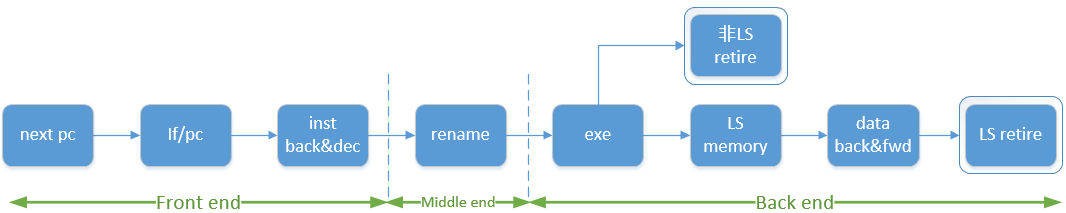
\includegraphics[width=\linewidth]{figs/pipeline.png}
	\caption{处理器流水线大致示意图}
\end{figure}
\section{前端的设计--性能和电路延迟都可以做到极优}
前端包括取指器,转移猜测器以及L1 cache,下面就从这三个角度来剖析:
\subsection{取指器--一个高效简洁优美的模型实现}
工程的方法学就是从简单到复杂。而最简单的就是宽度为1的取指器,代码如下:
\begin{scala} 
	val sWtAddrOK :: sWtInstOK :: sWtForward :: Nil = Enum(3)
	switch (state) {
		is (sWtAddrOK) {
			when(addr_ready) { state := sWtInstOK }
		}
		is (sWtInstOK) {
			when(inst.valid) {
				when(io.forward || inst_kill) {
					state := Mux(addr_ready, sWtInstOK, sWtAddrOK)
				}.elsewhen(io.dec_kill) { state := sWtAddrOK
				}.otherwise { state := sWtForward }
			}
		}
		is (sWtForward) {
			when(io.forward) {
				state := Mux(addr_ready, sWtInstOK, sWtAddrOK)
			}.elsewhen(io.dec_kill) { state := sWtAddrOK }
		}
	}
\end{scala}
上面的代码就是描述整个取指器行为的状态机,一共只有3个状态,非常的简洁清晰。用图来描述就是:
\begin{figure}[H]
	\centering
	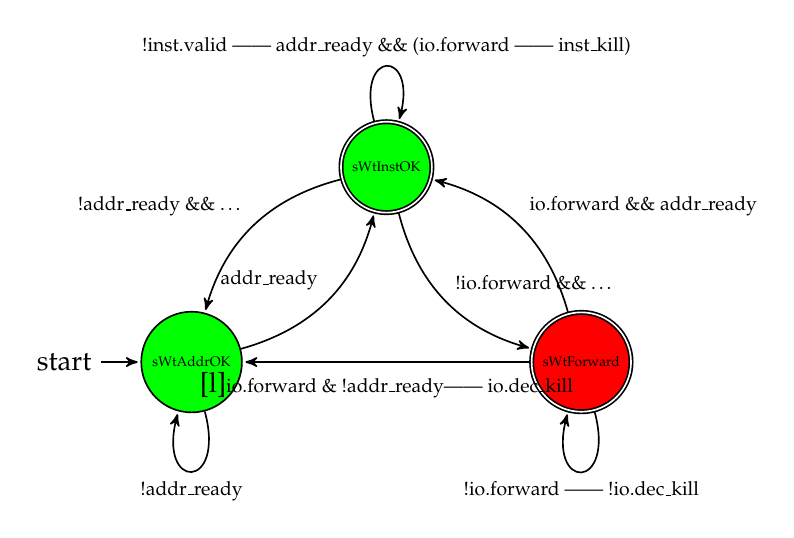
\begin{tikzpicture} [->,>=stealth',shorten >=1pt,auto,node distance=3.5cm,
	semithick]
	\node[state, accepting, fill=green](q0) {\tiny{sWtInstOK}};
	\node[state, below left of=q0, initial,fill=green] (q1) {\tiny{sWtAddrOK}};
	\node[state, accepting, below right of=q0,fill=red](q2) {\tiny{sWtForward}};
	
	\path
	(q1) edge[bend right] node{\scriptsize{addr\_ready}} (q0) 
	edge[loop below] node{\scriptsize{!addr\_ready}} ()
	
	(q0) edge[bend right] node[swap]{\scriptsize{!addr\_ready \&\& \dots}} (q1) edge[bend right] node{\scriptsize{!io.forward \&\& \dots}} (q2) edge[loop above] node{\scriptsize{!inst.valid || addr\_ready \&\& (io.forward || inst\_kill) }} ()
	
	(q2) edge[bend right] node[swap]{\scriptsize{io.forward \&\& addr\_ready}} (q0) edge node{\Longstack[l]{\scriptsize{io.forward \& !addr\_ready} \\ \scriptsize{|| io.dec\_kill}}} (q1)
	edge[loop below] node{\scriptsize{!io.forward || !io.dec\_kill}} ();
	\end{tikzpicture}
	\caption{the FSM of FetchInst module}
\end{figure}
然后再辅以三大控制变量来配合这状态机就可以完整地刻画取指器的行为了:
\begin{scala}
	io.inst.valid := (inst.valid && !inst_kill)|| state === sWtForward
	
	pc_valid := state === sWtAddrOK || (state === sWtForward && io.forward) ||
	(inst.valid && (io.forward || inst_kill))
	
	io.pc_forward := io.if_kill || (addr_ready && pc_valid)
\end{scala}
这3个控制变量非常重要,因为它背后代表的是一个三级流水的模型,而且这个3级流水的inflight的指令只有1条。见下图,3级分别是next\_pc, if/pc, inst back\&dec
\begin{figure}[H]
	\centering
	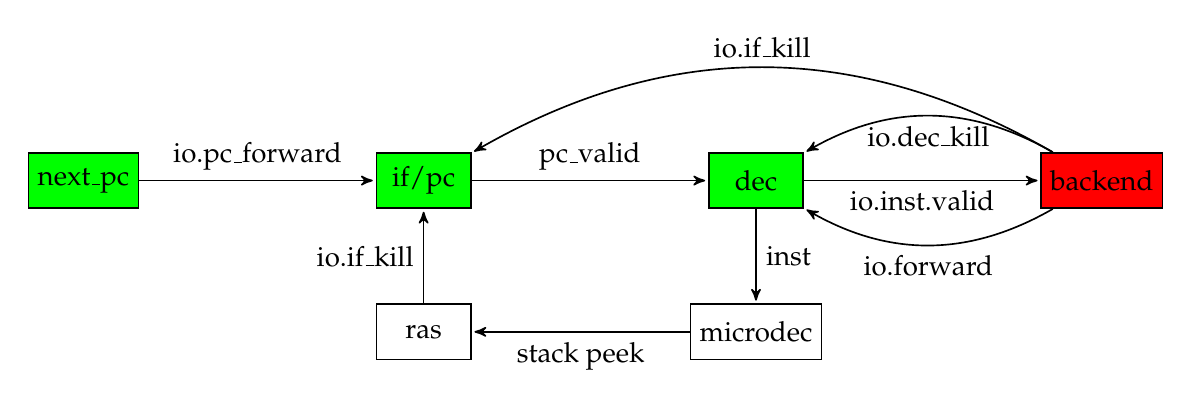
\begin{tikzpicture}[
	node distance = 12mm and 30mm,
	->,>=stealth',shorten >=1pt,semithick,
	box/.style = {rectangle, draw, fill=#1, 
		minimum width=12mm, minimum height=7mm}
	]
	
	\node (n1) [box=green] { next\_pc };
	\node (n2) [box=green,right=of n1] {if/pc};
	\node (n3) [box=green,right=of n2] {dec};
	\node (n4) [box=red,right=of n3] {backend};
	\node (n5) [box=white,below=of n3] {microdec};
	\node (n6) [box=white,below=of n2] {ras};
	%
	\draw[->] (n1) to ["io.pc\_forward"] (n2);
	\draw[->] (n2) to ["pc\_valid"] (n3);
	\draw[->, swap] (n3) to ["io.inst.valid"] (n4);
	\draw[->, bend left] (n4) to ["io.forward"] (n3);
	\draw[->, bend right,swap] (n4) to ["io.if\_kill"](n2);
	\draw[->, bend right] (n4) to ["io.dec\_kill"] (n3);
	\draw[->] (n3) to ["inst"] (n5);
	\draw[->] (n5) to ["stack peek"] (n6);
	\draw[->] (n6) to ["io.if\_kill"] (n2);
	\end{tikzpicture} 
	\caption{the pipeline of frontend}	
\end{figure}
io.pc\_forward是控制相应信号从next\_pc级流向if/pc级的闸门,也就是使能信号,pc\_valid是控制相应信号从if/pc级流向dec级的闸门,io.inst.valid和io.forward组合起来控制相应信号从dec级最后流向backend进行处理。最后还有辅以io.if\_kill和io.dec\_kill是的前端支持cancel机制。这3级流水的阻塞与流通解释起来非常简单,首先最靠近后端的dec级如果在inst.valid和forward同时置上的时候,才能被后端接收,下一拍空出这一级,而if/pc级的信号要流向dec级必须等到dec级在下一拍是能够被空出来的,同理next\_pc级的信号要流向if/pc级必须要等到if/pc级在下一拍能够被空出来的。inflight的指令数为1的含义需要解释一下,指的是在途的访问memory或者cache的pc至多为1,或者可以理解为要等到dec级的inst被backend接收,if/pc级的pc才能够被置为有效。这个基本的限制非常重要,重要到如果没有这个限制假设,整个取指器的模型将不会这么优美,复杂性会大大提升,甚至会控制不住。

值得一提的是,这个发射器的频率能达到很高,原因在于,所有后端和memory传来的信号,都是用锁存器锁一拍再利用的,而且由于模型简单,附加的逻辑门级不多,这样可以把物理的延迟降到最低。频率就可以做到极限。

\subsection{取指器宽度从1到2的跨越}
所以从1到2的跨越是最难的。这是因为从1到2是一个质的飞跃不是一个量的积累。也在设计的时候意识到了上面做出的假设模型的伟大之处,使得不仅宽度2取指逻辑的在复杂度上得到了控制,做到在逻辑上基本上和宽度1相当,而且还充分发挥了宽度为2的优势。不过首先需要撇清的一个误区是,由于外围memory的端口宽度是不易修改的,所以如果直接访问memory,那么回来的指令宽度仍然是1而不是2,所以不同于cache命中一下能取回两条指令,像cache miss后直接访问memory指令是一条一条回来的。我设计的取指器在面对这种情况的时候,也是会一条接一条往后端发送,不会等着两条指令同时取回来再发送。另外,这也在一方面说明在通常意义上实现超标量都是要带指令cache的。如下是宽度为2的取指器的状态机:
\begin{scala}
	val sWtAddrOK :: sWtInstOK :: sWtForward :: Nil = Enum(3)
	val state = RegInit(sWtAddrOK)
	val inst_valid_orR: Bool = inst_valid.reduce(_||_)
	val if_forward: Bool = io.forward(1) || inst_kill || Mux(inst_split, io.pc(conf.pcLSB).toBool, !inst_valid(1))
	switch (state) {
		is (sWtAddrOK) {
			when (addr_ready) { state := sWtInstOK }
		}
		is (sWtInstOK) {
			when(inst_valid_orR) {
				when(if_forward) {
					state := Mux(addr_ready, sWtInstOK, sWtAddrOK)
				}.elsewhen (io.dec_kill) { state := sWtAddrOK
				}.otherwise { state := sWtForward }
			}
		}
		is (sWtForward) {
			when(io.forward(1)) {
				state := Mux(addr_ready, sWtInstOK, sWtAddrOK)
			}.elsewhen (io.dec_kill) { state := sWtAddrOK }
		}
	}
\end{scala}
状态机的跳转表如果画出来和宽度为1的时候相似,而且就连状态数都没有增加一个,这是一个很了不起的结果。毫不夸张的说,取指器的设计把效率和频率兼得地都发挥到了极致,而且是基于如此简单的模型,如此简洁的代码。
虽然宽度2的代码基本照搬宽度1,但是仍有几个需要比宽度1多考虑的逻辑:
\begin{enumerate}
	\item 首先超标量的第一条指令一定要是偶数的指令,第二条一定要是奇数的指令。如果if/pc级发出偶数的pc,然而dec级由于cache miss再通过burst传输先传回了第一条偶数的指令,这时候可以不用管forward的信号,立马发出后一条的奇数的pc取指。这个考虑使得无论再什么样的情况下,宽度2的取指器效率都不会低于宽度1的取指效率。
	\item 其次指令流会有跳转,而且有一半的概率是在第一条指令的后面需要跳转,这种情况被我叫做inst split,代码中就是用inst\_split变量来表示,如果第二条指令也取回来了,要取消掉
	\item 为了继续提高效率,还用了一些小技巧。一般来说除了两条连续的偶数奇数的pc之间连续取指不用顾及后端的forward信号,其他时刻都必须等到前端的inst valid和后端的forward信号握手fire之后,才能够继续取指,也就是inflight指令只能为1的设定。但是有一种情况例外,就是如果第一条是跳转指令,而且转移预测器预测到要跳转而且跳转的pc是奇数,也可以马上去取指,不用顾及后端forward的情况。
\end{enumerate}
而且秉承了宽度为1的取指器留下的优良传统,凡是外部发来的信号对于取指器状态都会延后一拍做出相应的改变,这样可以做到取指器的时序独立于外部的时序。

\subsection{cache core设计}
数据和控制应该相互独立,这是设计中最为基本也是最重要的哲学思想,这也是为什么cache core要独立出来讲的原因。它可以有不同的数据组织形式,可以是直接映射的,可以是全相连的,也可以是多路的。多路的时候也可以有不同的替换算法。但这一切都与怎么读写的逻辑无关,对外呈现的只有读写端口。只要求cache行的长度对外保持一致即可。将数据和控制逻辑解耦和,可以做到最大程度控制复杂度。另外一方面同时也可以做到逻辑的复用。比如icache和dcache对于读写的控制不一样,但是cache core的存储逻辑可以做到一致。截至中期,工程实现依旧采用的是直接映射的存储结构,后期会将其调整为4路组相连结构。这里有两个目的。其一,risc-v对于页表的规定固定为4KB,为了做到cpu的tlb虚实转化和访问cache的并行,所以cache core的每一路的容量都至多是4KB,也就是说用虚实地址共享的地址(不用tlb cam来进行虚实转换)来索引cache core。但是4KB的容量显然不够的,但是每一路至多4KB,当然可以用硬件来解决顶着色对每一路的cache core进行扩容,但是这就很复杂了。所以另一种思路就是增加路数,比如四路;其二,四路比一路cache的替换率要低,这不光是容量的问题,四路的每路4KB的cache在一般情况下要比容量相同的16KB的单路cache的替换率都低。

所以对于cache core最终的组织形式目前的想法是4路组相连,每一路4KB,采用LRU或者随机替换或者一种兼而有之的方法。不会参考alpha21464一样做路预测,一是为了降低复杂度,二是因为估计在自己的设计中延迟时序允许。
\subsection{icache的设计--一个高效简洁而优美的设计实现}
沿袭了龙芯杯上的简洁高效的设计,如下是icache的状态机代码:
\begin{scala}
	val sLookUp :: sBurst :: sWriteBack :: Nil = Enum(3)
	val state = RegInit(sLookUp)
	switch (state) {
		is (sLookUp) {
			when (pc_miss) { state := sBurst
			}.otherwise { state := sLookUp }
		}
		is (sBurst) {
			when (rlast && rvalid) { state := sWriteBack
			}.otherwise { state := sBurst }
		}
		is (sWriteBack) {
			when (pc_double_miss) { state := sBurst
			}.otherwise { state := sLookUp}
		}
	}
\end{scala}

状态机一共有3个状态,一个是lookup阶段,也就是在icache查找pc对应的指令是否命中,如果出现miss了就进入burst状态进行burst传输。burst传输是AXI协议中的一种传输模式(但也不局限于AXI协议),就是发出一个pc,能够取回来与这个PC相关一连串的指令,一旦burst传输回来,就是一排一条指令,比方说burst的长度设置为16,即使cache miss,在一段访问memory延迟后,也有16个周期是有指令可以提供的,这样就能够大大降低访存延迟的代价。所以icache就把burst传输设置为16,与icache的cache line长度吻合。其实在AXI协议中burst还有着两种基本的模式,一种是INCR,一种是SWAP。通俗来说INCR就是在以PC为起点,往后取一段指令,所以INCR发出的PC一般要以要去的指令长度对其。SWAP同样是以PC为起点,但是PC不要求是指令宽度中最前段的指令,可以是中间的某条指令,然后可以做到到达要求边界后再折回来取从最头上取指直到取回来pc的前一条。目前的设计中,icache采用的是INCR模式,因为其一取指有连续的倾向,而且在很大的情况下导致burst传输的pc都是cache line的第一条,虽然SWAP模式一定不会比INCR差,但是SWAP模式其实和INCR差不多;其二,考虑到取值时序紧张,INCR模式对内对外都比SWAP模式友好,所有最后采用的INCR模式。回到状态机上,当状态是burst时,如果rlast和rvalid信号同时置上了,说明最后一条指令也被取回来了,状态就会跳到writeback状态。writeback状态下就是把取回来暂时缓存的整个cache line写回cache core中。为了提高效率,在burst传输阶段也是同步可以消化取回来的指令的,这样就会出现可能一个跳转出现第二次的pc miss,这个时候整个取指器就会卡住动不了了,因为这第二次的cache miss要等到前一个的burst传输完,对应的指令才被取回来,这个是之前提过的三级模型中就已经强调过的。而在writeback阶段如果检查到pc double
miss就会直接又进入下一个的burst传输阶段,提高效率。如果没有出现二次miss,那么就会又跳回lookup状态。
整个状态机用图表示如下所示:
\begin{figure}[H]
	\centering
	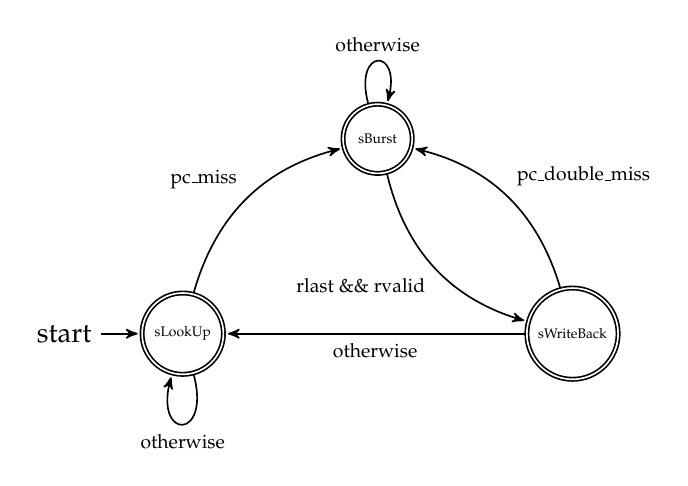
\begin{tikzpicture} [->,>=stealth',shorten >=1pt,auto,node distance=3.5cm,
	semithick]
	\node[state, accepting](q0) {\tiny{sBurst}};
	\node[state, below left of=q0, initial, accepting] (q1) {\tiny{sLookUp}};
	\node[state, below right of=q0, accepting](q2) {\tiny{sWriteBack}};
	
	\path
	(q1) edge[bend left] node{\scriptsize{pc\_miss}} (q0) 
	edge[loop below] node{\scriptsize{otherwise}} ()
	(q0) edge[bend right] node[swap]{\scriptsize{rlast \&\& rvalid}} (q2) 
	edge[loop above] node{\scriptsize{otherwise}} ()
	(q2) edge[bend right] node[swap]{\scriptsize{pc\_double\_miss}} (q0) 
	edge node{\scriptsize{otherwise}} (q1);
	\end{tikzpicture}
	\caption{the FSM of Icache module 注意到每一个状态都可以作为结束状态}
\end{figure}
\subsection{多级的转移预测器\chinesedash 面积,时序,正确率的综合考虑}
除了cache,转移猜测也是高性能CPU的关键。与简单的流水线后端一遇到阻塞就要暂停取指器的取指不同,高性能的处理器后端一定不是这样做的,因为瓶颈已经摆在那里了,所以一定是要做到遇到阻塞比如访存指令地址miss有数十拍的延迟,还能允许前段正常取指。言下之意就是后端要有一个自身的缓存指令的机制,在一些处理器中也被称为指令的inflight。既然是缓存指令,那也就是不会马上被执行,所以也就不知道跳转的真正结果。但是平均6$ \sim $ 8条指令中就会有一条转移指令,如果没有转移猜测,一味的增加pc,那么基本上后面取到的指令基本上都是错误的,等到前面的跳转指令被执行了,后面的指令又会被cancel掉,体现不出指令缓存的作用,反而浪费面积。要真正发挥缓存指令的优势,就必须靠转移猜测来提高缓存队列中指令的正确性。但如果细细分析一下,指令的猜测可以分为好几级:
\begin{enumerate}
	\item if/pc级就要得到next pc,此时还不知道pc对应的指令是不是跳转指令,所以构唯一的映射关系是pc到next pc。但是pc毕竟有32位,靠ram来索引显然不符合实际,剩下的方案只有cam表比较了,代表性的数据结构是就是BTB。而且cam也只能存少数的映射关系,比如32个,64个。
	\item dec级这个时候指令已经取回来了,但是整个周期的延迟也就够把指令取回来再做简单的译码,最多只能够做根据译码结果得到是ra指令选择ras的栈顶地址。
	\item 五级流水中对应的exe级在五级流水中就直接运算得到了跳转地址,但是在更高性能的处理器中,流水级切得更多的情况下,这一级被用作rename还来不及运算执行。对于简单的jal指令,可以直接由对应的pc和指令中的立即数域得到跳转地址并反馈到前端预测器。而对于branch类指令,虽然能够算出跳转地址,但是不知道跳与否。这个时候可以用BHT的数据结构和gshare之类的hash算法来猜跳或不跳。
\end{enumerate}

转移猜测中有很多取舍的考虑,如果想把预测率做高,就要付出面积,电路延迟,级数,功耗的代价。商用的处理器的转移猜测正确率能够达到95\%,但是这不意味着他们的预测器猜对了就一个周期都不损失,不可能。(光光靠第一级的BTB运行一般程序能够达到95\%的正确率是不可能做到的,但是pc级又确实就只能够靠BTB来进行简单的映射猜测)这就意味着如果下游的猜测机制检测到流水线上游猜的不对,纠正的时候也要损失周期数。

这就是目前在我的设计中转移猜测这三级的考虑。

目前截至中期,只实现了pc级的带两位饱和计数器的BTB和dec级的ras纠正。ras比较简单,就是一个栈的结构,针对的是函数调用的情况,一遇到要跳转到函数的指令,就把其pc+4压入栈中,一遇到函数返回的指令,就弹栈。在顺序中没有什么困难的,但是乱序中就有问题了,什么时候入栈,什么时候出栈。是猜测的时候?还是真正执行完的时候,可是如果是乱序的后端,又怎么保证初入栈的顺序,或者为了简单干脆就不保证了?

另外一个数据结构BTB原理也不困难,但是却是转移猜测中最为重要的一个部件,直接分担了80\%多的正确率。虽然BTB就是一个记录了跳转分支指令的pc到其要跳转的target的一张cam表,但是为了使得这张表整体更加高效,意味着要延迟更小,表的容量更大,正确率更高,面积更小的综合目标。所以对这个逻辑上简单的从pc到target的映射关系,我们要好好的分析一下从而得到更好的物理实现。首先观察到的一点就是在映射关系中,无论是pc还是target的高位很少有变化,几乎是不变的,所以一个想法就是能不能把高位比如说高20位和低位比如低12位分开,做成两个表的映射。这样考虑到高位不怎么变动,那么高位的表就可以做的项数少一点比如4项。低位就可以做的相对多一点,比如64项。可以计算一下,如果采用如上的设计方案,总共占用的面积是$ 4\times20\times2 + 64\times12\times2 + 64\times2 = 1824 $比特,最后加的64×2是索引高位cam表的index的所需要的面积,这个相当于29项直接32位pc映射到32位target,如果是64位的isa下,这种优势会更加明显。也就是面积一样,在理想情况下容量提高到只有一张cam表的的2倍多。那么电路延迟如何呢?面积一样的情况下,两张cam表的延迟不会比一张cam表差。其中两张cam表中最占时间的是64项12位cam的比较,相较于一张cam表的29项32位cam的比较,延迟是占优。
\begin{figure}[H]
	\centering
	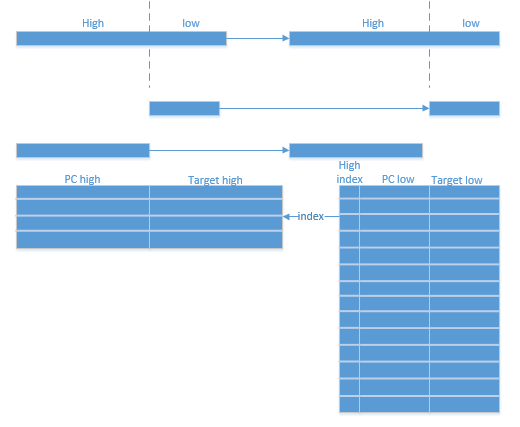
\includegraphics[width=0.45\linewidth]{figs/btb1.png}
	\caption{观察1引出的物理数据结构的优化}
\end{figure}
观察到的第二点就是pc到target的映射中高位基本上都是一致的,也就是程序的行为大多数都是在小范围内相对跳转的。针对这一特点,在低位的映射表中再加1bit的标志位,标记映射的高位是不是相等,这样如果高位相等就不需要去占用高位cam表的一项了,大大降低了高位cam表的替换率,从而提高了预测率。
\begin{figure}[H]
	\centering
	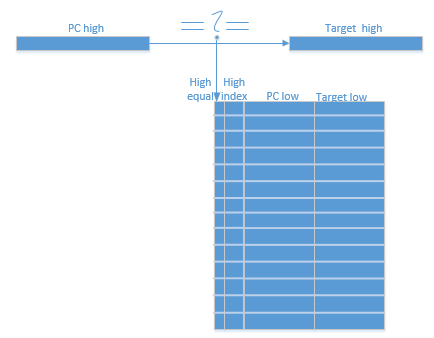
\includegraphics[width=\linewidth/2]{figs/btb2.png}
	\caption{观察2引出的物理数据结构的优化}
\end{figure}
第三个观察是jump类的指令是肯定会跳转的,但是分支类的指令可能跳也可能不跳,如果完全猜测跳的话显然不合理,所以参考BHT,这里引入两位饱和计数器,操作与BHT一致。同时为了区分jump类的指令和branch类的指令,这里用2bit来标注不同的跳转指令类型:
\begin{scala}
	object BTBType {
		val invalid = 0
		val retn    = 1
		val branch  = 2
		val jump    = 3
		val NUM = jump + 1
		val SZ = log2Ceil(NUM)
	}
\end{scala}
这里的类别中还把jump类的指令细分为了return类指令和普通jump,这是因为return指令是通过寄存器跳转的,而且代码的不同位置都可以调用函数,所以return类的指令的跳转target经常是会变动的,所以在BTB中的target参考意义不大,但是函数调用有非常好的栈的特性,就可以用ras栈顶的target作为next pc,这样能提高return指令的预测率。所以最后的低位cam表就是表7所呈现的形式。

这样就基本论述了前两级的转移猜测技术,事实上目前我也只做了这些。不过目前在代码框架的设计上我也考虑到了一些能够在未来加入的更为复杂和精确预测策略的例如在第二级和第三级联动用BHT和gshare算法。事实上一些由于可能存在的指令的修改导致不是转移指令出现BTB预测跳转和branch指令跳转target发生离奇错误的纠正逻辑已经在第二级第三级有所实现。但是目前来说,我的着力点还是先将乱序实现,观察一下乱序的效果,然后才会考虑结合着对程序跳转行为的分析把转移猜测做得更好。
\begin{figure}[H]
	\centering
	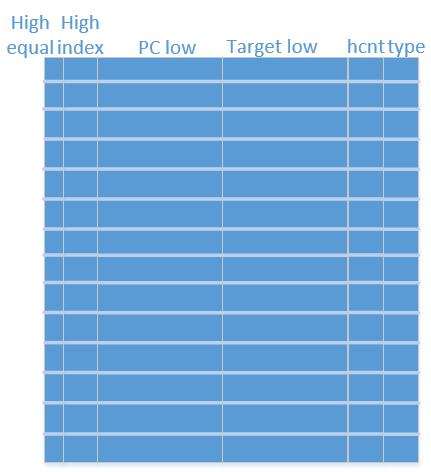
\includegraphics[width=0.5\linewidth]{figs/btb3.png}
	\caption{观察3引出的低位cam表的改进}
\end{figure}

\subsection{前端部件的整合}
上面讲述了前端的各个组件,接下来就是把这些组件拼接起来。对于一条指令宽度的前端非常的简单,但是对于两条指令宽度的前段,就要考虑两条并行的指令的干扰问题,说的更具体一点就是第一条指令对第二条指令的影响。仔细分析一下前段流水线的每一级:
\begin{enumerate}
	\item 第0级$ \chinesedash $ next\_pc级是没有的这种现象的,因为next\_pc只有一条
	\item 第1级$ \chinesedash $ if/pc级开始有这种现象,虽然对外的取指端口还是一个pc,但是这个时候对内的pc已经分化成两个,一个是偶数的pc,一个是紧接着的奇数的pc。这样在BTB的结构中,如果第一条pc在btb表中命中,而且其映射的target作为下一条pc就不是连续的,加之最后的预测的结果是跳转的话,那么第二条奇数的pc就会被无效掉。这个问题在取指器FetchInst模块已经解决。
	\item 第2级$ \chinesedash $ dec级,产生指令之间影响的原因有两种,其一,同样与转移预测有关,如果dec级的转移预测器对于dec级第一条指令的next pc预测信息产生了区别于if/pc级的预测信息,那么就要将与之同时取回的第二条指令无效掉;其二,为了使得后端的逻辑简单化,decorde出来两条都是特权指令或者两条都是分支跳转指令时,就要强行将其拆成一拍一个地发向后端
	\item 第3级$ \chinesedash $ rename级,转移预测器如果在这一级的第一条指令上又纠正了上一级预测的错误。同样要将与之并行的第二条指令无效掉。
\end{enumerate}
\section{中间层的设计}
中间层包括了许多物理部件,有专属于中间层的前端指令队列,分支跳转预测队列,也有和后端共享的发射队列,分支跳转队列和访存队列,作为入口处为这些队列提供相应的数据。也有对整个CPU状态总体控制的控制单元和实现精确发射的机制。在讨论每个物理部件之前,要先提的是这些物理部件的承载抽象的数据结构--队列。而队列有两种实现形式:
\begin{enumerate}
	\item 循环队列,依靠着两组指针分别是是head和tail来控制逻辑。称之为组是考虑到同时入队列和同时出队列的不止一项。入队列移动tail,出队列移动head。
	\item 移位队列,只需要依靠一个计数器来记录当前队列中有多少项即可,入队列从队列的尾部依靠计数器来进入;出队列的项的后面诸项需要向前移位来填补出队列的项的空白。
\end{enumerate}
\begin{figure}[H]
	\centering
	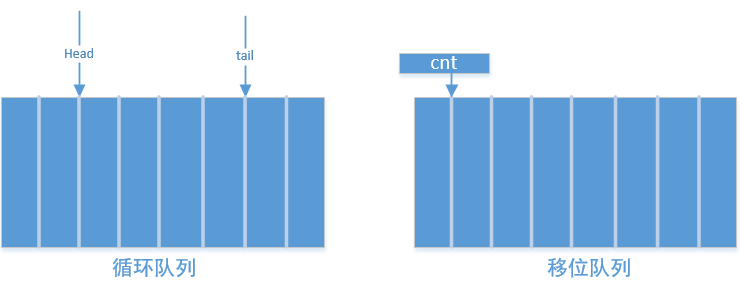
\includegraphics[width=0.7\linewidth]{figs/fifo.png}
	\caption{两种队列示意图}
\end{figure}

这两种物理实现形式各有优势。循环队列对于出入队列的项数约束较松,能耗较低,只需要移动指针即可;移位队列对于出队列的项数约束较严,一般入队的项数多少不会影响到移位队列的物理实现复杂度,但是对于出队的项数,一项是最为简洁的,但是一旦项数大于1,复杂度就会明显地提高,物理实现变得困难,同时移位队列的功耗比循环队列大不少,因为平均1/2项数都会变动。但是循环队列并不适合承载乱序的逻辑,同样是由其逻辑特性决定的,因为出队列只能从head开始;而移位队列却非常适合承载乱序的逻辑,因为出队不一定要从最头部,同时乱序中如果存在多项同时可以出队,但是只能选最早一项的逻辑,移位队列处理起来也非常的简洁优美,选距离头部最近的一项即可。但是移位队列的功耗毕竟太大,特别是每一项位数很大的时候。出于降功耗的考虑,对移位队列的结构做了优化如下图所示:
\begin{figure}[H]
	\centering
	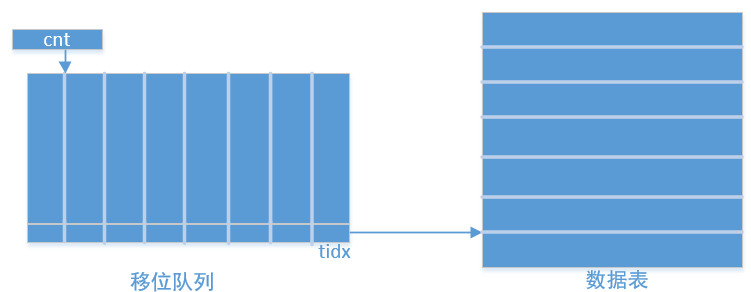
\includegraphics[width=0.7\linewidth]{figs/fifotable.png}
	\caption{移位队列加数据表的结构示意图}
\end{figure}
只将影响到弹出队列条件的最关键控制信号填入移位队列中,其他相关的数据信号填入到数据表中,然后把该表项的索引同时填入移位队列中。出移位队列时再用这个索引去索引数据数据表得到数据。

整个中间层和后端就是用这两个最为基本的数据结构组合起来的。如果用这种视角去设计乱序多发射处理器,将会最大限度的控制复杂度。但是复杂度依然很大,如果把整个设计都事无巨细的表达出来,将会是长篇累牍的,从阅读的角度来看并不会达到很好的效果。所以为了避免做过于复杂的阐述,对下面的每个物理部件都进行了很大程度的逻辑简化。
\subsection{前端指令队列}
前面提到了高性能的CPU一定是有不包括cache在内的指令缓存的,同时前面也提到了指令的执行优先级划分的合理性。所以在我的设计中采用了两种不同形式的指令缓存。其中一种的执行优先级较低,主体部分位于第2级inst back\&dec,采用循环队列顺序缓存指令,称之为前端指令队列。
\begin{figure}[H]
	\centering
	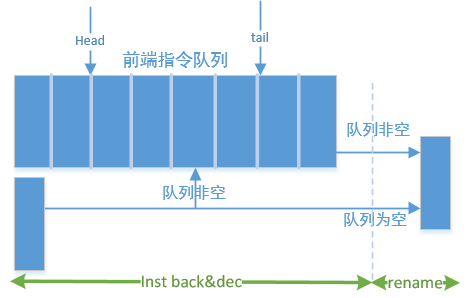
\includegraphics[width=0.7\linewidth]{figs/frontqueue.png}
	\caption{前端指令队列示意简图}
\end{figure}
队列的每一项能够容纳两条指令,与取指器的宽度相符。从取指器取回来的两条指令在至少有一条是有效的情况下,如果下游rename级没被阻塞并且队列为空,直接在下一周期进入rename级,否则进入队列,队列满时阻塞前端取值。队列项数目前设计为16项,也就是说容量是32条指令,能够抵挡16个周期的下游阻塞。
\subsection{分支跳转预测队列}
从前端传来的不仅有指令,同时也有转移猜测的信息。直观上来讲,转移猜测的信息的存储格式和前端指令队列一致,但是仍有几点不同,导致了最后结构的差异:
\begin{enumerate}
	\item 在前面前端部件整合中提到的解决并行的两条指令的干扰问题的机制使得同一周期中间层最多接收到1条分支跳转指令,所以预测队列每项的宽度为1即可。
	\item 由于中间层处于流水线第三级,而转移猜测也可以做到第三级,如果提前在第二级就把预测信息存入队列做到和前端指令端队列一样,然后再在第三级做必要的修改就会有些麻烦。所以做成预测信号在第二级仍然能够经过预测器变换修正传到第三级再写入队列中反而是更加合理的选择。最后只需要保证出队列的指令和出队列的预测信号是一一对应的即可。
\end{enumerate}
\begin{figure}[H]
	\centering
	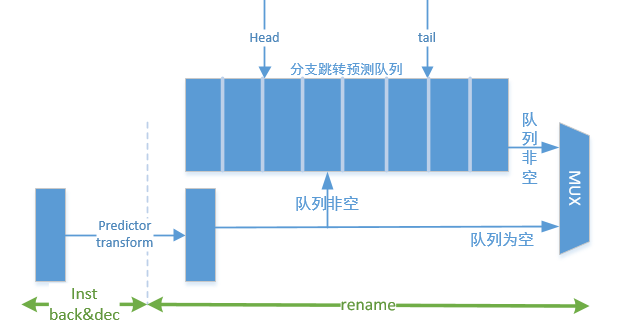
\includegraphics[width=0.7\linewidth]{figs/predqueue.png}
	\caption{分支跳转预测队列示意简图}
\end{figure}
\subsection{为什么不需要PC队列}
前端传来的不仅有指令,转移猜测信息,还有PC,直观来看也应该有一个PC队列来存放pc信号。但是仔细一想,每一周期的pc其实是可以由预测队列得到的,因为预测队列里存放的正好是下一周期的PC值。所以没有必要把pc存起来。这同样也降低了处理器面积的开销,想想如果把32条pc都存放起来了,面积就和regfile相当了。
\subsection{发射队列}
前面只说了前端指令队列这一种指令缓存的形式,这另外一种就是发射队列,发射队列的执行优先级较高,为第二梯队,物理位置紧挨着前端指令队列的下游,要求乱序执行,所以用移位队列就非常合适。但是移位队列对于出队列的项数要求非常严格,以1项为最佳。所以做了两个平行的发射队列,对应前端队列每一项的两条指令,都是一进一出的移位队列。
\begin{figure}[H]
	\centering
	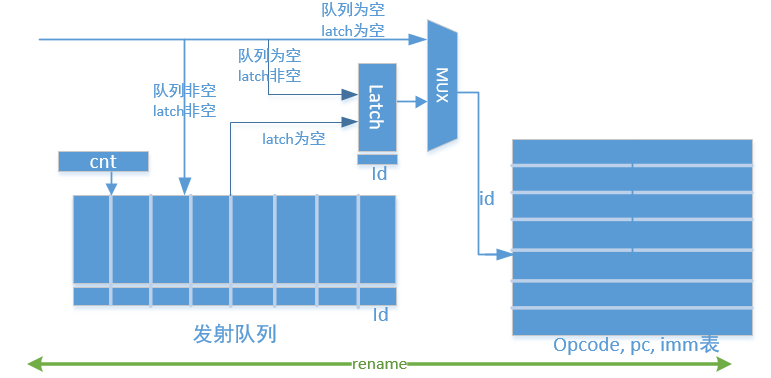
\includegraphics[width=0.7\linewidth]{figs/instqueue.png}
	\caption{发射队列示意简图}
\end{figure}
为了规整,移位队列主体为8项凑足2的幂次,但是又为了扩容,也为了从结构上更加顺畅,又加了一项的latch,在发射队列里的指令发射的时候会先在下一周期进入这个latch,然后这个latch去regfile读取操作数并同时用id索引所需要的pc,操作码,立即数(译码是在第3级rename级进行的,所以这个时候指令已经被译码,立即数、pc、执行微码被存入表中,同时注意到第二种形式要存放pc,因为指令执行是乱序的,要区别于之前讲的第一种指令缓存形式不用存PC的技巧)。这样两个并行的发射队列的容量是18条指令。
\subsection{CPU状态控制单元}
之前有第4章节已经阐述和强调了什么是CPU的状态。那么理解CPU的状态为什么有那么重要,因为它是整个处理器核心设计中的核心,无论是顺序的CPU,超标量的CPU,乱序的CPU,本质上都在做一件事,那就是根据指令正确的改变CPU的状态。所以高性能的CPU以一种更高的角度来看就是能够更高效的改变自身状态的CPU。而且乱序中最大的挑战也在于由于转移猜测错误,或者是中断例外到来而要引起的CPU状态的精确还原,还原到引发猜测错误的那条转移指令的状态现场,还原到中断例外发生所以之前指令都提交的状态现场。或者更具体一点,因为乱序要依靠寄存器的重命名技术,要怎么做到围绕着重命名表的精确回退机制。这里有两种大的方向,一种是基于cam的重命名机制,一种是基于ram的重命名机制。我目前的设计采用的是后者ram,因为ram相较于cam更加直观,逻辑也更加简单。下面就是围绕着ram重命名表在我的设计中的state表示
\begin{scala}
	class State(val nEntry: Int) extends Bundle {
		val useing = UInt(nEntry.W)
		val usecnt = UInt(log2Ceil(nEntry+1).W)
		val maptb  = Vec(32, UInt(log2Ceil(nEntry).W))
		val rename = Vec(32, Bool())
	}
\end{scala}	
基于ram的重命名表在上述代码中就是maptb变量,nEntry是物理寄存器堆的项数,所以log2Ceil(nEntry)就是索引物理寄存器堆地址的位数。目前的设计将nEntry定为60.其他变量的含义分别是
\begin{enumerate}
	\item useing: 正在使用的物理寄存器分布向量,每一个物理寄存器占一位,1表示正在被使用,0表示空闲,可以被分配。
	\item usecnt: 正在使用的物理寄存器计数器,能够产生分配物理寄存器的ready信号,比如需要分配一个物理寄存器需要usecnt < nEntry才行。
	\item rename: 逻辑寄存器号是否已经被映射到某一个物理寄存器号,如果是则为1,不是为0。含义是清晰的,但是让人费解的是为什么会有这个变量。简单的解释就是这个变量是用于回收过时的物理寄存器的。
\end{enumerate}
所以有了这么一个状态的刻画,需要有多少个不同的状态就可以new多少个这个state class。首先要有一个最新的状态,负责当前的重命名和物理寄存器号分配。其次为了能够在中断例外来的时候恢复到之前所有指令都已经commit的状态,还应该有一个记录commit的状态。然后比如我的设计中最多支持4个跳转分支指令猜测执行,那么就需要4个备份来应对不同的猜测错误的现场恢复。对应的代码如下:
\begin{scala}
	val latest = RegInit({
		val w = Wire(new State(nPhyAddr))
		w.maptb  := DontCare
		w.useing := 0.U
		w.usecnt := 0.U
		w.rename := VecInit(Seq.fill(32)(false.B))
		w
	})
	val commit = RegInit({
		val w = Wire(new State(nPhyAddr))
		w.maptb  := DontCare
		w.useing := 0.U
		w.usecnt := 0.U
		w.rename := VecInit(Seq.fill(32)(false.B))
		w
	})
	val backup = Reg(Vec(nBrchjr, new State(nPhyAddr)))
\end{scala}	
有了状态的描述,回溯恢复操作基本上就是把相应要回溯的状态变量赋值给latest状态即可(这里略去一下复杂的更新修改细节),非常的简单直观。

下来回到控制逻辑本身。作为状态的总控单元,两大最主要的功能
\begin{enumerate}
	\item 指令id号的分配,背后的载体是reorder buffer,简称为ROB,组织形式是循环队列,id号从tail分配,从head顺序回收。
	\item 物理寄存号的分配,背后的载体是物理寄存器堆。分配的时候找从左边数的第一个1,从右边数的第一个1,这样就可以做到并行同时最多能够分配两个物理寄存器号。
\end{enumerate}
指令id是标记处理器乱序部分顺序的唯一标志。不同于cam形式的重命名机制下还需要带有分支id,在ram形式的重命名机制下,唯一的id号足够了。这也是ram比cam简洁的一个地方。在我的设计中,id是5位的,所以也就意味着我的处理器乱序部分最多支持32条乱序的指令。
\subsection{分支跳转队列}
分支队列和访存队列就是面向后端的数据结构,所以在中间层的章节里只是顺带提一下,在后面章节$ \chinesedash $后端设计中会有详细的说明。首先分支跳转队列的入口在中间层,说明是顺序地分配相应的资源,换句话说,分支跳转队列不是执行时才分配的。原因很简单,因为分支跳转是控制相关的,自带顺序属性,也就是说乱序中也要保持相对的顺序,这一点和发射队列很像。所以分支队列的入口所在的流水级和发射队列是一致的。采用的数据结构组织形式也和发射队列类似,都是移位队列,如下图:
\begin{figure}[H]
	\centering
	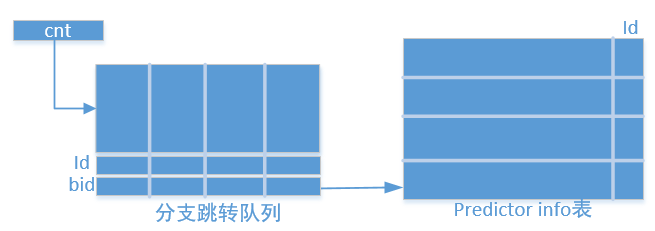
\includegraphics[width=0.7\linewidth]{figs/branchqueue.png}
	\caption{分支跳转队列示意简图}
\end{figure}
\subsection{访存队列}
这里需要阐明两点。其一,直观来讲,访存指令并不是控制相关的,那么为什么也要求顺序的时候分配相应的资源呢?其二,如下图给出的访存队列数据控制组织结构,为什么却不是类似于发射队列和分支队列一样采用的移位队列而是用循环队列呢?。核心的原因在于:对比普通寄存器数操作指令,写后写,写后读的冲突可以由重命名机制来很好的解决,但是重命名机制却做不好访存指令的写后写,写后读冲突,因为访存的地址不是在重命名的时候得到的,而是在乱序的执行阶段得到的,乱序就没有了次序,没有了次序也就不知道指令先后了,也就无法检测访存指令之间写后写,写后读的冲突。所以为了解决这个问题,这里就必须用队列的物理属性顺序分配来对保持访存指令的顺序行控制。另外,队列类型的选择不用移位队列而采用移位队列的原因在于:为了判读写后写,写后读的冲突,整个32位或者64位地址都将是关键信号(store的数据可以不是),也要在移位队列中进行移位,如此一来功耗将会非常高。其次,还有一个更为重要的原因,因为store的写操作是对外的,所以已经超出了之前所讲的CPU状态控制的范畴,要实现精确例外,store指令必须要等到前面所有的指令确定不发生例外在能够顺序的把数据写回内存中,这是一个顺序的逻辑,天然的适合用循环队列来做。load队列确实可以做成移位队列,做到乱序出队列。但是因为平均而言,load指令占整个指令总量的15\%左右,如果从功耗的开销和所获得的收益的角度来考虑,做成8项或者6项的循环load队列已经大概率的满足32条指令乱序执行中的load指令地址和其他控制信号的存放。所以做成移位队列获得的性能上的收益微乎其微,并不值得去实现。
\begin{figure}[H]
	\centering
	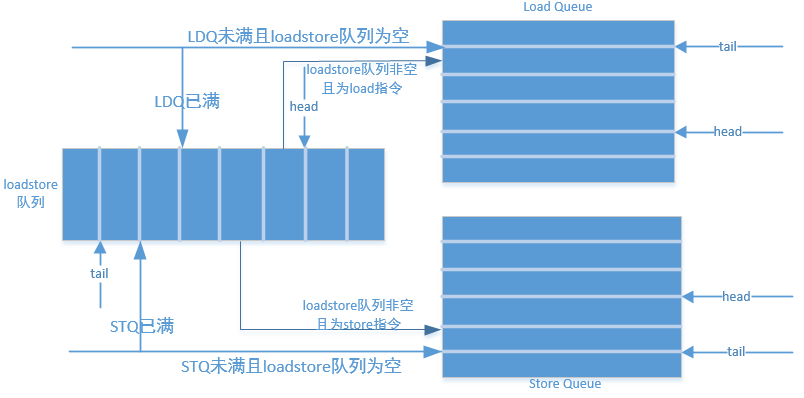
\includegraphics[width=0.7\linewidth]{figs/loadstqueue.png}
	\caption{访存队列示意简图}
\end{figure}
\subsection{精确发射}
在中间层的设计过程当中,会发现精确发射的逻辑也是非常的复杂。精确发射,指的就是综合各个物理部件剩余容量和指令对各个物理部件资源的需求完全精准的来得到指令是否能够发射的条件。这个问题的复杂性在于
\begin{enumerate}
	\item 不同指令的需求是不一样的。有的指令有写寄存器的需求,所以需要分配物理寄存器;有的是跳转分支指令,在分支队列要分配项数;有的是访存指令,需要在访存队列中分配项数。
	\item 同一指令的需求是多样的,可能既需要物理寄存器,也需要访存队列
	\item 需要对两条并行的指令进行同时分配,第一条指令的分配情况会组合逻辑的作用于第二条指令发分配情况。所以并行的指令如果要实现精确分配物理资源就必须是串行和顺序的。
\end{enumerate}
所以很多发射宽度更高比如四发射的处理器都采用了保守发射的逻辑,只要指令有效,就认为指令有所有的需求,换言之就是只需要关心指令是否有效即可,就是为了避免其复杂性。另外,在复杂处理器的设计中,由于各个部件的面积都很大,布局布线的位置也会相隔较远,所以若采用精确发射走线延迟也很大。但是本身我的处理器设计面积就不是很大,资源队列的项数相对较小,走线延迟不算很大,而且另一方面项数小就要节约着用,所以权衡之下才用精确发射会提高资源的利用率和执行的效率。

仔细分析,在我目前的设计中中间层需要分配的资源有五个,分别是:
\begin{enumerate}
	\item 指令标识符id       每条指令都必须分配,最多需要分配2项
	\item 物理寄存器号       有写寄存器的需求的指令分配,最多需要分配2项
	\item 发射队列entry     发射队列是两个并行独立的,所以每个队列最多秩序分配1项。目前的设计是除了特权态指令不需要进如发射队列发射指令,其余的用户态指令需要分配。
	\item 访存队列entry     访存指令需要分配,最多分配2项
	\item 分支跳转队列entry  分支跳转指令除了jal指令都需要
\end{enumerate}
再进一步的解耦和观察,一方面是两条并行指令的各个需求以及是否有效,另外一方面是各个物理部件的容量信息,如下图:
\begin{figure}[H]
	\centering
	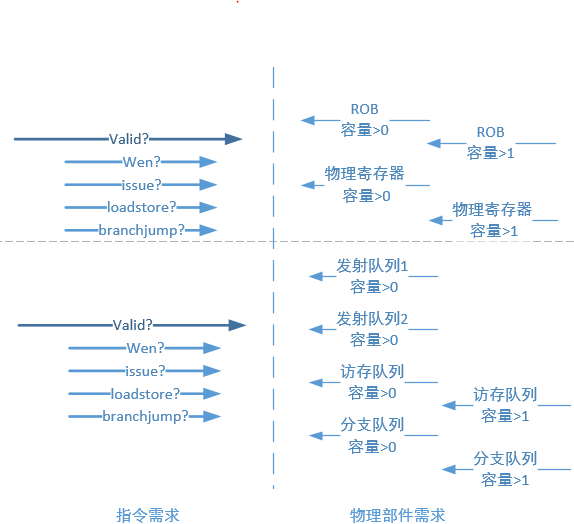
\includegraphics[width=0.6\linewidth]{figs/issue.png}
	\caption{精确发射分析}
\end{figure}
\section{后端的设计}
前文已经提到过,中间层缓存了32条顺序指令,而后端则缓存了32条乱序指令,这种设定直观上来看是非常合理的。
\subsection{发射队列}
采用移位队列图9的组织形式,顺序入队乱序出队,实现了乱序化的第一步。在移位队列中的信息可以精简到两个物理寄存器号带上是否需要继续侦听的标志位,加上一个用来索引数据表的id号大概总共20bit每项,所以移位所产生的功耗还是得到控制的。
\subsection{执行队列}
这个队列就是上文提及的执行等级的第一梯队,组织的格式同样是图9的移位队列,而且移位队列中entry的内容和发射队列保持一致,物理上就可以保证指令的相对顺序。缺点很明显$ \chinesedash $面积开销很大,但是优点同样明显,执行快而且不需要读寄存器堆,将物理寄存器堆的读端口维持在4个,物理布局布线能够接受的水平。执行队列还有一个很重要的功能是及时平衡发射队列的指令数量。因为两个发射队列是独立平行的,每个队列只分别负责接收从前端送来的两条指令的有效的第一条和第二条。由于并不是每个周期的两个指令都是有效的,所以会导致发射队列指令数不平衡,影响到资源的利用率。依靠执行队列,当执行级两条指令同时因为操作数没有准备号被阻塞住时,接受来自含指令条数多的发射队列的那一条指令,从而起到平衡发射队列的作用。
\subsection{分支跳转部件}
主体是分支跳转队列,对接着前端的转移预测器,构成了整个反馈回路的分支跳转系统。这一系统在高性能处理器的重要性仅次于访存系统。高性能的分支跳转系统在设计的时候有3大指标需要考虑:
\begin{enumerate}
	\item 高准确率  是设计的首要指标,90\%的准确率下处理器的IPC和95\%的准确率下的IPC都要相差很多
	\item 低周期数  同样是设计中要考虑的重要指标。举例来说,如果A款处理器的命中率是95\%,但是反馈周期是6(反馈周期按我的定义是从投机的取跳转指令的下一周期的指令开始,到跳转指令被执行能够发出重定向信号为止,一共需要经过多少个周期)。B款处理器的命中率是90\%,但是反馈周期是3. 在不考虑指令缓存的更为复杂的因素下,A、B处理器预测效果是差不多的。
	\item 低延迟,小面积,低功耗
\end{enumerate}
而在分支队列的设计中,主要对应的指标就是低周期数。分支队列的结构如图13所示,目前的设计中有4项,也就是说乱序的32条指令中允许有4条分支,这四条分支能够把整个指令流分成5段,所以每段的平均长度在$6\sim7$之间,恰好也符合跳转分支指令在总指令中的平均占比。回到图13,会发现和图9的标准移位队列有些出入。主要体现在的地方是分支队列和分支信息表都多了id域(bid是需要的,因为要索引数据表)。移位队列要有id域是由于中间层就要分配,但是后端的执行是乱序的,执行完成回到分支队列就要用到cam查找去匹配到属于自己的那一项entry,然后再靠对应的bid来索引table得到相应的信息。理论上还存在着另外一种方案,就是ram查找,如果用ram,就必须在每一条指令都带上bid,比cam逻辑麻烦,而且分支跳转队列只有4项,算得上项数很少了。

table中的id域的作用同样是为了cam查找。这个id域是可以不要的,因为可以先通过cam索引移位队列得到对应的bid然后再去索引table。但是如果加上id域,就意味着两个结构的查找可以做到并行。这并行的考虑正是为了降低反馈周期数而专门设计的。反馈做到可以走组合逻辑路线的就不走时序逻辑路线。什么情况下可以用组合逻辑而又不影响CPU整体的延迟。仔细分析一下,除了jr类指令需要读取寄存器来进行运算,其他的分支跳转指令都是直接通过pc和指令中的立即数域进行符号拓展就可以得到跳转地址的,所以到中间层的时候跳转地址就能够被计算出来,顺势就可以存入分支表中。而且还需要注意的是像j类指令直接知道跳转地址和一定要跳的指令,是不会进入分支队列的,在risc-v中只有branch和jr两类指令会进入队列。在执行级,branch真正做的操作只有两个操作数的比较,工作量相对较少,所以就非常适合组合逻辑直接反馈;而jr类指令因为要算地址,所以先进入队列和表项中,然后在下一周期再对前端做出反馈。
\subsection{访存部件}
访存部件的主体是3个循环队列组成,分别是LDQ,STQ和load/store队列,在重命名阶段分配,每个队列的每项都带有全局id,后端的每个流水级利用cam查找到队列中对应的项并做出更新。LDQ和STQ意义和功能都非常明确,资源的释放也都是在load和store指令commit的时候。但是被称为load/store队列的这第三个队列又有什么设计上的考虑和用意。

引入这第三个队列的考虑在于:凡是在中间层分配的队列资源,都有一个缺点,就是只要存在指令有入队列的请求,但是队列已满,那么后端就会一律暂停接收来自前端或者中间层前端指令队列的指令。所以跳转指令和访存指令都存在这个问题。对于跳转指令而言,由于是控制相关的,维护起来代价巨大,不易做多,不得不牺牲这方面的考量。而访存指令的情况又不同于跳转指令,首先是一长串的连续的访存指令不少见,尤其在访存密集的程序中,6项的LDQ或者6项的STQ如果遇到这种情况不够用,就必须阻塞后面的指令。但此时有可能发射队列还很空,例如也就6条load指令分散于两个之中,也就是每个队列3条,乱序资源得不到有效的利用,所以有必要对LDQ和STQ扩容;但是另外一方面,在一长串的访存类指令中,一般都是处于同一或者相邻cache行的,所以真正需要长时间在执行中的访存指令也相对较少,不宜对LDQ和STQ扩容,增加无谓的面积去存储肯定暂时得不到的地址数据。

综上所述,现在面临的两难局面是:一边为了提高乱序资源利用率而主张扩容,一边为了不增加访存队列面积而反对扩容。解决的方案就是增加一个load/store队列。这个队列里每一项的信息非常少,只有一个id,一个访存类型,一个load/store标记位。这个队列做到8项,占用的总资源也不会超过80bits,非常的小巧。这第三个队列和STQ和LDQ的交互大致是如图14所示,load/store指令会优先选择进入STQ或者LDQ,只有到LDQ或者STQ满了,才会填入load/store队列。而STQ或LDQ释放的资源后也会优先分配给load/store队列中的项,如果queue是空的,才会直接填入从中间层送来的访存指令信息。同时为了逻辑的正确性,必须规定凡是在这个loads/tore队列里的指令不能够被发射执行,直到该条访存指令被转移到了LDQ或者STQ,才能重新获得被发射的权利。load/store队列加上这个规定,将会提高处理器在运行访存密集程序上的性能。

访存部件涉及到后端所有的流水级,而且又是与CPU的外部信号交互,是后端中最复杂的一个部件。列举每一级的操作:
\begin{enumerate}
	\item rename级$ \chinesedash $ 访存指令进入相应的队列
	\item exe级$ \chinesedash $ 计算出访存的地址写入相应的队列中
	\item LS memory级$ \chinesedash $ 向外发出load请求,并且遍历队列得到写后读的相关forward信号
	\item data back\&fwd级$ \chinesedash $ 数据load回来,进行必要的forward操作,练到写回总线
	\item LS retire级$ \chinesedash $ 如果是load指令直接retire;如果是store指令往memory写完数据之后retire,同时store要做相关的backward操作,判读是否与已经取指回来的load指令有写后读的冲突,以便作必要的回滚。
\end{enumerate}
上述只是粗略的说明,并不准确,也省略了很多细节。由于写后读的冲突的存在,使得STQ和LDQ虽然是两个队列但有着密切的关联。维护这种联系的被我叫做forward和backward的两种操作。forward操作的主体是正要访存的load指令,动作是在STQ中前向扫描在该load指令之前的store指令,如果有地址冲突,store的数据就要前递到load的数据域中。backward的操作主体是处在STQ队列头部的store指令,动作是在LDQ中后向扫描在该store指令之后的load指令,如果存在读写地址冲突的情况,并且对应的load指令并没有来得及完成forward操作,就要向CPU状态总控单元发出回滚的请求。如下图所示:
\begin{figure}[H]
	\centering
	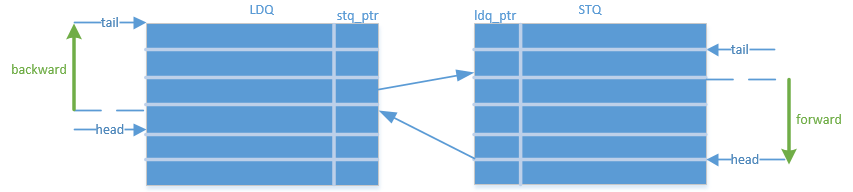
\includegraphics[width=\linewidth]{figs/fwdbwd.png}
	\caption{forward \& backward示意图}
\end{figure}

为了确定forward和backward的起点,在原来的队列中各要加入指针域,在LDQ中是索引STQ的指针stq\_ptr,在STQ中是索引LDQ的指针ldq\_ptr。
\subsection{特权态指令执行的初步方案}
前面提到的后端各个数据结构大多都是针对用户态指令的,而特权态指令相对稀少而且特殊,目前还没有来得及针对risc-v好好分析一下特权态指令的依赖关系来进行优化,初步的方案是特权指令一律不会进入发射队列乱序化,而且一定要等到ROB为空时才能够直接发射执行。
\subsection{后端状态回溯机制}
状态的回溯在前面中间层的CPU状态控制单元已经有所提及,除了CPU状态控制单元负责CPU状态的回溯以外,对于后端其他数据结构的状态回溯因为有一个很好的抽象也就显得非常的简单直观。这是因为后端和中间层都是由队列构成的,或者是移位队列或者是循环队列。对于移位队列,如果是例外中断或者访存回滚,计数器置为0即可;如果是跳转指令取缔,将计数器置为id号小于该跳转指令的指令个数。对于循环队列,同理操纵head和tail指针即可。
\section{处理器执行流回顾和电路延迟分析}
前端的章节中已经提到取指器的时序非常好,所有从后端传递的反馈信号都是锁一拍才会对取指器产生作用。而BTB也对其数据结构做了相应的物理的优化。前端是3级的流水,指令在第3级产生,被送到连接前后端的中间层,中间层先经过重命名把逻辑寄存器地址转化为物理寄存器地址,紧接着去索引物理寄存器堆读取数据出来直接送到锁存器,或者其实物理寄存器可以做成一个同步ram。CPU的最长路径极有可能会是这一条,目测估计要经过34级们左右。与这条路径并行的是物理资源的分配以及精确发射。如果发射队列为空就直接可以进入执行级执行,否则先进入发射队列轮循侦结果总线和旁路总线的信号。结果总线顾名思义就是结果已经得到的写回信息,而旁路总线指的是当前正要被发射,正在重命名读寄存器送到exe级执行的信号,换言之是预言下一拍就会得到结果的前递信号。由于commit总线的宽度是4,regfile的的写端口是4个,所以两类前递总线各有4组,总共8组。前递逻辑是时序也是比较紧张的,目测和中间层逻辑门级数要少一两级,但是相差不大。执行级依据内部微码对操作数进行运算,当然被送到exe级存在操作数还没有准备好的情况,将其压入执行队列。但是执行队列限定每一次只允许一条指令入队。处于平衡队列的考虑,如果同时出现两个发射队列的头部都没有准备好操作数,优先选择指令条数多的队列的头部指令入队。对于跳转指令和访存指令这种特定类别的指令执行控制,参考9.3,9.4章节。

\section*{\huge{二、下一步的工作计划与内容}}
代码逻辑上后期首要做的工作还有:
\begin{enumerate}
	\item 采用更加复杂的转移猜测策略,提高预测正确率
	\item 将icache从单路改成4路
	\item 将dcache改为写回模式,并从单路改为4路
\end{enumerate}

在已有的risc-v+chisel的工程框架下,针对risc-v32i的isa,把乱序双发射处理器在软件模拟层面调试成功。同时按照国科大结构实验课的方案,使得自己的处理器能够在FPGA平台上将测试程序跑通,做到真正的硬件正确。接着再进行对嵌入式benchmark程序的性能统计、评测,分析其乱序的调度的效率以及调度策略的合理性,做出一些优化。电路延迟方面,要结合综合布局布线工具对时序进行评测、优化与磨合。

最后,如果是以设计出一款能够运行程序的双发射乱序处理器为参加答辩的最低标准,目前觉得能够按期答辩。

\section*{\huge{三、已取得研究成果列表}}
无
\includepdf[pages={3},scale=1.1]{zhongqi.pdf}

\section{利用高级语言的优势来降低逻辑的复杂度}
\section{乱序调度的注意点}
发射队列的乱序调度基本是是保证相对顺序的调度,也及如果准备好了操作数的指令,会依靠物理结构的便利来选出其中最早的一条指令执行。只要发射队列不空而且队列头能够空出来,就能够从队列弹出一条指令。这条指令有两种可能的情况,一种是操作数都已准备就绪,发射出去执行即可。另一种是操作数没有准备好,但也被发射出去了,或者说发射出去才发现操作数没有准备好,会进入执行队列。执行队列和发射队列是一对一的valid,ready模式,所以握手的逻辑比较清晰。执行队列也是相对有序的,所以如果两个并行的发射队列的发射的指令操作数都没有准备好,会挑选两者中更早的指令进入执行队列。但是上面将的两种情况中都有一种例外需要用额外的逻辑来处理。第一种,操作数已经准备就绪,但不是最早的指令,这种情况会发生在访存指令有发射的限制上。第二种,操作数没有准备就绪,但不是最早的指令,这种情况会发生在访存指令miss了,也就是说发射完了才知道。
\section{chisel模块级调试的陷阱}
printf对于wire类型的变量和reg类型的变量的处理是不一样的,也就是说翻译为的verilog再进行仿真出来的效果是有区别的。呈现出的效果用一个例子来说明的话,就是如果把一个wire类型的变量赋值给reg类型,printf出来的两个变量的值变化是同步的,这个是非常不符合电路的规律的。也就是说reg类型打印出来的是input端的值的变化,这一点要尤其注意。
\end{document}
